\documentclass[letterpaper,10pt]{article}

\usepackage{geometry}
\usepackage{titlesec}
\usepackage{listings}
\usepackage{color}
\usepackage{hyperref}
\usepackage[nopostdot]{glossaries}
\usepackage[pdftex]{graphicx}
\usepackage{tikz}
\usepackage{wrapfig}
\geometry{textheight=8.5in, textwidth=6in}
\newenvironment{bottompar}{\par\vspace*{\fill}}{\clearpage}

\titleclass{\subsubsubsection}{straight}[\subsection]
\titleclass{\subsubsubsubsection}{straight}[\subsection]

\newcounter{subsubsubsection}[subsubsection]
\newcounter{subsubsubsubsection}[subsubsubsection]
\renewcommand\thesubsubsubsection{\thesubsubsection.\arabic{subsubsubsection}}
\renewcommand\thesubsubsubsubsection{\thesubsubsubsection.\arabic{subsubsubsubsection}}
\renewcommand\theparagraph{\thesubsubsubsection.\arabic{paragraph}} % optional; useful if paragraphs are to be numbered

\titleformat{\subsubsubsection}
  {\normalfont\normalsize\bfseries}{\thesubsubsubsection}{1em}{}
\titlespacing*{\subsubsubsection}
{0pt}{3.25ex plus 1ex minus .2ex}{1.5ex plus .2ex}

\titleformat{\subsubsubsubsection}
  {\normalfont\normalsize\bfseries}{\thesubsubsubsubsection}{1em}{}
\titlespacing*{\subsubsubsubsection}
{0pt}{3.25ex plus 1ex minus .4ex}{1.5ex}

\makeatletter
\renewcommand\paragraph{\@startsection{paragraph}{6}{\z@}%
  {3.25ex \@plus1ex \@minus.2ex}%
  {-1em}%
  {\normalfont\normalsize\bfseries}}

\renewcommand\subparagraph{\@startsection{subparagraph}{7}{\parindent}%
  {3.25ex \@plus1ex \@minus .2ex}%
  {-1em}%
  {\normalfont\normalsize\bfseries}}

\def\toclevel@subsubsubsection{4}
\def\toclevel@subsubsubsubsection{5}
\def\toclevel@paragraph{6}
\def\toclevel@paragraph{7}

\def\l@subsubsubsection{\@dottedtocline{4}{7em}{4em}}
\def\l@subsubsubsubsection{\@dottedtocline{5}{9em}{5em}}
\def\l@paragraph{\@dottedtocline{6}{10em}{6em}}
\def\l@subparagraph{\@dottedtocline{7}{14em}{7em}}
\makeatother

\setcounter{secnumdepth}{5}
\setcounter{tocdepth}{5}

\definecolor{codegreen}{rgb}{0,0.6,0}
\definecolor{codegray}{rgb}{0.5,0.5,0.5}
\definecolor{codepurple}{rgb}{0.58,0,0.82}
\definecolor{backcolour}{rgb}{0.95,0.95,0.92}
 
 \lstdefinestyle{mystyle}{
backgroundcolor=\color{backcolour},   
commentstyle=\color{codegreen},
keywordstyle=\color{magenta},
numberstyle=\tiny\color{codegray},
stringstyle=\color{codepurple},
basicstyle=\footnotesize,
breakatwhitespace=false,         
breaklines=true,                 
captionpos=b,                    
keepspaces=true,                 
numbers=left,                    
numbersep=5pt,                  
showspaces=false,                
showstringspaces=false,
showtabs=false,                  
tabsize=2
}

\lstset{style=mystyle}

\makeglossaries
\loadglsentries[main]{Glossary}

\title{Final Report For RockSat-X Payload - Hephaestus}
\author{Helena~Bales, Amber~Horvath, and Michael~Humphrey\\ \\ CS463 - Spring 2017}

\parindent = 0.0 in
\parskip = 0.1 in

\begin{document}
\maketitle

\begin{abstract}
The \gls{osu} RockSat-X team shall be named Hephaestus.
The progress of our project shall be outlined in this document.
The mission requires that the \gls{payload}, an autonomous robotic arm, perform a series of motions to locate predetermined targets.
The hardware shall be capable of performing the motions to reach the targets.
The software shall determine the targets and send the commands to the hardware to execute the motion.
The combination of the hardware controlled by the software shall demonstrate Hephaestus's ability to construct small parts on orbit.
\end{abstract}

\begin{center}

\includegraphics[scale=.03]{logo}

Hephaestus Mission Logo
\end{center}

\begin{bottompar}
Approved By - Dr. Nancy Squires
\_\_\_\_\_\_\_\_\_\_\_\_\_\_\_\_\_\_\_\_\_\_\_\_\_\_\_\_\_\_\_\_\_\_\_\_\_\_\_\_\_\_\_\_\_\_\_\_\_\_\_\_\_\_\_\_\_\_\_\_\_\_\_
Date \_\_\_\_\_\_\_\_\_\_\_\_\_\_\_\_\_\_\_\_\_\_\_\_\_\_\_\_ \\


Approved By - Helena Bales
\_\_\_\_\_\_\_\_\_\_\_\_\_\_\_\_\_\_\_\_\_\_\_\_\_\_\_\_\_\_\_\_\_\_\_\_\_\_\_\_\_\_\_\_\_\_\_\_\_\_\_\_\_\_\_\_\_\_\_\_\_\_\_\_\_\_\_\_\_\_
Date \_\_\_\_\_\_\_\_\_\_\_\_\_\_\_\_\_\_\_\_\_\_\_\_\_\_\_\_ \\


Approved By - Amber Horvath
\_\_\_\_\_\_\_\_\_\_\_\_\_\_\_\_\_\_\_\_\_\_\_\_\_\_\_\_\_\_\_\_\_\_\_\_\_\_\_\_\_\_\_\_\_\_\_\_\_\_\_\_\_\_\_\_\_\_\_\_\_\_\_\_\_\_\_
Date \_\_\_\_\_\_\_\_\_\_\_\_\_\_\_\_\_\_\_\_\_\_\_\_\_\_\_\_ \\


Approved By - Michael Humphrey
\_\_\_\_\_\_\_\_\_\_\_\_\_\_\_\_\_\_\_\_\_\_\_\_\_\_\_\_\_\_\_\_\_\_\_\_\_\_\_\_\_\_\_\_\_\_\_\_\_\_\_\_\_\_\_\_\_\_\_\_\_\_\_
Date \_\_\_\_\_\_\_\_\_\_\_\_\_\_\_\_\_\_\_\_\_\_\_\_\_\_\_\_ \\
\end{bottompar}

\clearpage
\tableofcontents
\clearpage

\section{Introduction}
The Hephaestus project is a 2016-2017 Senior Design project involving seniors
from the Computer Science, Electrical Engineering, and Mechanical Engineering 
disciplines. 
The project is a proof-of-concept for construction in a space-like environment.
The concept that we have chosen to pursue will be described over the course of 
this document but is, at its core, a high \gls{dof} robotic arm mounted on a 
rocketry \gls{payload}. 
At the next level of detail, the Hephaestus \gls{payload} is an autonomously 
controlled 4 \gls{dof} steel arm capable of precise, collisionless operations 
in \gls{microgravity} and vacuum conditions. 

This concept will be proven in August, following the 2017 RockSat-X launch from
\gls{wff} in West Virginia. 
RockSat-X is an educational ride-sharing program for student exploration of Low
Earth Orbit. 
The RockSat-X program is run by the Colorado Space Grant Consortium and 
provides students with a standard rocketry platform for space experiments.
This will be Oregon's first participation in the program, and \gls{osu}'s first
space mission.
This project is also supported by the \gls{osu} \gls{aiaa} club.

The success of this project will be determined following the launch in August.
Due to gravity, we are unable to test the function of the arm on earth.
The weight of the motors prohibits the arm from moving, even using a plastic 
version of the arm segments to reduce weight. 
Success of the mission will be measured in several ways.
The most direct way that we will see our success is by recording a video of the 
\gls{payload}'s operation on orbit using a GoPro camera. 
We will also receive telemetry data during the flight about the experiment's 
state and status of the on-board touch sensors. 
Finally, we will be storing data throughout the experiment to the \gls{obc} for
evaluation after the rocket's recovery.

The success of this mission will show the success of the Hephaestus Senior 
Design groups, take a step towards proving the viability of construction
on orbit using a small autonomous robotic arm, and show \gls{osu}'s ability to
put an experiment in space. 
The goal for this project is mission success and technical and professional 
development.

\subsection{Document Overview}
TODO

\section{Project Overview}
\subsection{Project Purpose}
The \gls{osu} RockSat-X team will demonstrate that an autonomous robotic arm 
can locate predetermined targets around the \gls{payload} under 
\gls{microgravity} conditions by using precise movements.
The technical actions performed by this demonstration will illustrate a 
proof-of-concept for creating assemblies, autonomous repairs, and performing 
experiments in space.

\subsection{Mission Success Criteria}
The following criteria determine if the Hephaestus mission will be considered 
successful post-flight.
The minimum mission success criteria represent the lowest criteria to be met 
in order for the mission to be considered successful.
If the minimum mission success criteria are not met, then the mission may not 
be considered successful.
The maximum success criteria define the highest goals for the mission.
Fulfilling any or all of these criteria, in addition to the minimum success 
criteria, would constitute a highly successful mission.
The success of the mission shall be evaluated by means of video recordings 
recovered post-flight and telemetry data received during and after the flight.

\subsubsection{Minimum Mission Success Criteria}
\begin{itemize}
\item{The arm assembly body shall deploy and a video sweep shall be successfully recorded.}
\item{The arm assembly body shall be fully retracted after data collection.}
\end{itemize}

\subsubsection{Maximum Mission Success Criteria}
\begin{itemize}
\item{The arm assembly body shall deploy and a video sweep is successfully recorded.}
\item{The arm shall make contact with predetermined targets around the payload.}
\item{The camera shall record all instances of contact between the arm and the targets.}
\item{The arm assembly body shall be fully retracted after data collection.}
\end{itemize}


\subsection{Concept of Operations}
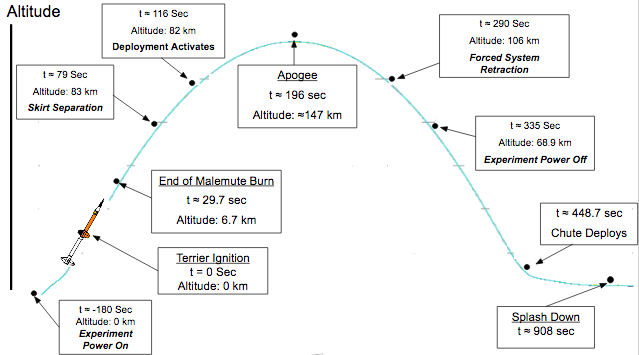
\includegraphics[width=\textwidth]{./images/conops}

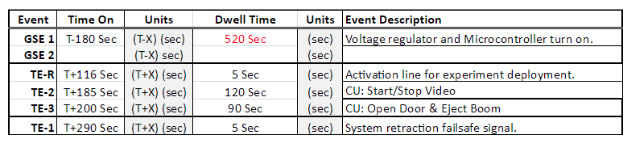
\includegraphics[width=\textwidth]{./images/conopsTable}
\begin{center}
	Concept of Operations for the 2017 RockSat-X Rocket Launch.
\end{center}

\subsection{Programmatics}
\subsubsection{Organizational Chart}
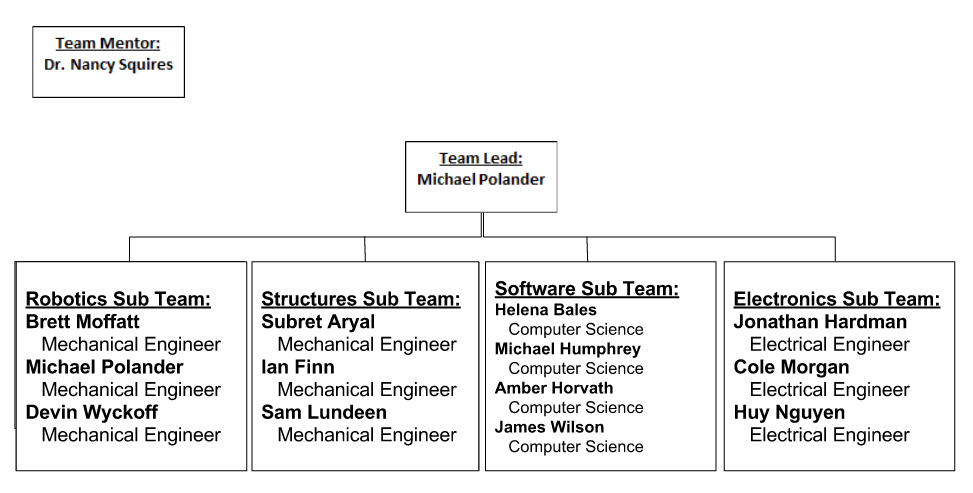
\includegraphics[width=\textwidth]{./images/orgChart.png}

\subsubsection{Sponsors}
The Hephaestus project is made possible by generous donations of time and money
from the following people and organizations:
\begin{itemize}
  \item{Dr. Nancy Squires, Techincal Advisor}
  \item{Oregon NASA Space Grant Consortium}
  \item{Colorado Space Grant Consortium}
  \item{\gls{aiaa}}
\end{itemize}

\section{Requirements Document}
\subsection{Original Requirements Document}
\subsection{Introduction}
\subsubsection{Purpose of Document}
This document shall describe in detail the Hephaestus RockSat-X payload.
It shall specify the software behavior of the payload.
This document will not discuss the specific implementations of the hardware or the software.
It will specify the behavior by describing the Functional and Non Functional requirements of the software.
This document will be updated throughout the project and should be considered a living document.

\subsubsection{Overview of Document}
This document will first cover the functional requirements of the project, then the non functional requirements.
The Functional Requirements will include descriptions of the main behavior, target generation, movement, operation modes, and telemetry.
Each of these topics will include descriptions of the behavioral requirements for each.
The Non Functional requirements will cover the performance, security, and telemetry.
Each of the non functional topics covered will include the requirements for the quality of each of the topics.

\subsubsection{Overview of Payload}
The Hephaestus RockSat-X payload is a deployable rocketry payload that will fly on the 2016 RockSat-X launch.
The payload's main function is to provide a proof of concept for delicate construction in a space environment.
The Hephaestus payload shall perform the following operations:
\begin{itemize}
\item{Remain retracted with power off for duration of launch}
\item{Power on at apogee}
\item{Deploy arm assembly body}
\item{Deploy arm}
\item{Perform 360 degree sweep with video camera}
\item{Generate targets for arm motions}
\item{Perform arm motions}
\item{Record each arm motion with video camera}
\item{Retract arm}
\item{Retract arm assembly body}
\item{Power off}
\end{itemize}

\subsubsection{Overview of Physical Payload}
While this document focuses on the software of the Hephaestus payload, the project also includes hardware
 and electrical systems. 
Understanding the physical appearance of the payload will help with understanding the software system. 
As such, Figure 1 should serve as a reference for the physical appearance of the payload.
\begin{figure}
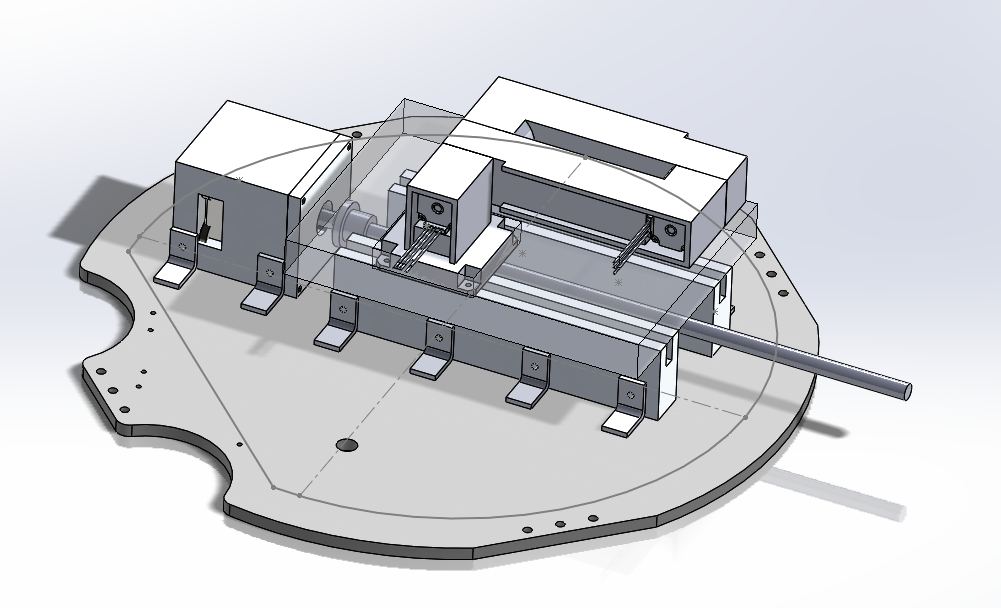
\includegraphics[scale=.5]{img2}
\caption{Model of Hephaestus Payload}
\end{figure}

\subsubsection{Mission Success Criteria}
The following criteria determine if the Hephaestus mission will be considered successful post-flight.
The minimum mission success criteria represent the lowest criteria to be met in order for the mission to be considered successful.
If the minimum mission success criteria are not met, then the mission may not be considered successful.
The maximum success criteria define the highest goals for the mission.
Fulfilling any or all of these criteria, in addition to the minimum success criteria, would constitute a highly successful mission.
The success of the mission shall be evaluated by means of video recordings recovered post-flight and telemetry data received during the flight.

\subsubsubsection{Minimum Mission Success Criteria}
\begin{itemize}
\item{The arm assembly body shall deploy and a video sweep is successfully recorded.}
\item{The arm assembly body shall be fully retracted after data collection.}
\end{itemize}

\subsubsubsection{Maximum Mission Success Criteria}
\begin{itemize}
\item{The arm assembly body shall deploy and a video sweep is successfully recorded.}
\item{The arm shall make contact with predetermined targets around the payload.}
\item{The camera shall record all instances of contact between the arm and the targets.}
\item{The arm assembly body shall be fully retracted after data collection.}
\end{itemize}

\subsubsection{Requirements Apportioning}

\subsubsubsection{Priority 1}
This is the highest priority level. In order for the software system to be considered complete and ready for launch, all requirements of this level must be met.
The completion of only Priority 1 requirements marks the completion of Minimum Mission Success criteria, as defined in subsection 1.4.

\subsubsubsection{Priority 2}
Requirements of Priority 2 are not required for the release of the software system.
Not completing these requirements must not present a risk to mission success.
The completion of these requirements and successful performance on orbit marks completion of part of the Maximum Success Criteria, as defined in subsection 1.4.

\subsubsubsection{Priority 3}
Requirements of Priority 3 are not required for the release of the software system.
Not completing these requirements must not present a risk to mission success.
Completion of all priority 3 requirements and those of higher priority, with successful performance on orbit, marks the completion of the Maximum Mission Success Criteria, as defined in subsection 1.4.

\subsection{Functional Requirements}

\subsubsection{Main Behavior}
\textbf{Priority 1:}
The software shall control the movement of the arm assembly body to make contact with the payload base
at locations generated by the Software (subsection 2.2). 

\subsubsection{Target Generation}
\textbf{Priority 1:}
The software shall generate points to be used in testing the Hephaestus arm.
The points will constitute the total test of the arm, and should therefore include points
representative of standard and edge cases.
The points shall be generated in polar form, including an angle from normal, a radius, and a height. 
The angle shall be in the range of 0 and 359 degrees.
An angle of zero degrees shall be in the direction of payload deployment.
The radius shall be the distance from the arm's attachment to the base to the generated point.
The height of the point, for the purpose of target generation, shall be constant.
However the points will always be stored in a triple of angle from normal (\(\theta\)), radius (\(r\)), and height (\(h\)).
These points shall be used as targets for the arm body.

\subsubsection{Movement}
The software shall control the movement of the arm body assembly. 
The position of the tip of the arm shall be tracked in the coordinate notation described in subsection 2.2 above.

\textbf{Priority 1:}
The software shall rotate the arm body assembly in a full 360 degrees.

\textbf{Priority 2:}
The software shall additionally control the movement the height of the arm body assembly.
The arm should descend and touch the baseplate of the payload at any rotation.

\subsubsection{Modes}
During the course of the flight, the software will progress though several different modes of operation.

\subsubsubsection{Launch}
\textbf{Priority 1:}
The software shall remain idle during launch.

\subsubsubsection{Deployment}
\textbf{Priority 1:}
The software shall power on the arm assembly body and video camera.
The software shall begin saving the video feed from the camera to a persistent storage location.
The software shall generate target points, as defined in subsection 2.2.

\subsubsubsection{Science}
\textbf{Priority 1:}
The software shall collect data to serve as a proof-of-concept for construction of structures in flight.

\subsubsubsection{Safety}
\textbf{Priority 1:}
The software shall ensure that the arm assembly body can be fully retracted after completing the mission.
The software shall, in case of a failure, eject the arm to prevent damage to the arm assembly body and the rocket during descent.

\subsubsubsection{Observation}
\textbf{Priority 1:}
The software shall report all telemetry data (as defined in 2.5) to the ground station.

\textbf{Priority 2:}
The software shall be responsible for turning the camera on and off.

\subsubsubsection{Power Off}
\textbf{Priority 1:}
The software shall power down all subsystems of the payload in preparation for descent.

\subsubsubsection{State Diagram}
\begin{center}
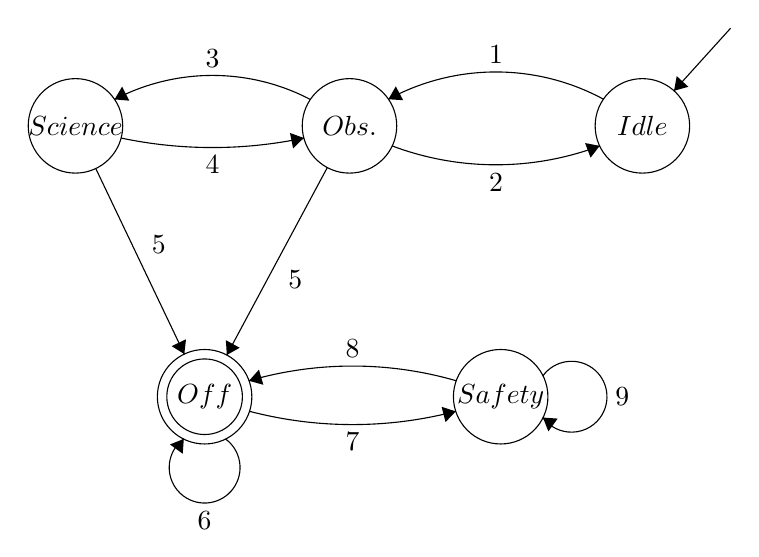
\begin{tikzpicture}[scale=0.2]
\tikzstyle{every node}+=[inner sep=0pt]
\draw [black] (24.2,-19.2) circle (3);
\draw (24.2,-19.2) node {$Obs.$};
\draw [black] (42.8,-19.2) circle (3);
\draw (42.8,-19.2) node {$Idle$};
\draw [black] (6.8,-19.2) circle (3);
\draw (6.8,-19.2) node {$Science$};
\draw [black] (15,-36.4) circle (3);
\draw (15,-36.4) node {$Off$};
\draw [black] (15,-36.4) circle (2.4);
\draw [black] (33.8,-36.4) circle (3);
\draw (33.8,-36.4) node {$Safety$};
\draw [black] (48.4,-13) -- (44.81,-16.97);
\fill [black] (44.81,-16.97) -- (45.72,-16.72) -- (44.98,-16.04);
\draw [black] (26.67,-17.507) arc (118.43354:61.56646:14.344);
\fill [black] (26.67,-17.51) -- (27.61,-17.57) -- (27.14,-16.69);
\draw (33.5,-15.28) node [above] {$1$};
\draw [black] (40.088,-20.475) arc (-69.41442:-110.58558:18.736);
\fill [black] (40.09,-20.47) -- (39.16,-20.29) -- (39.51,-21.22);
\draw (33.5,-22.17) node [below] {$2$};
\draw [black] (9.281,-17.525) arc (117.61533:62.38467:13.416);
\fill [black] (9.28,-17.52) -- (10.22,-17.6) -- (9.76,-16.71);
\draw (15.5,-15.5) node [above] {$3$};
\draw [black] (21.303,-19.973) arc (-78.10445:-101.89555:28.152);
\fill [black] (21.3,-19.97) -- (20.42,-19.65) -- (20.62,-20.63);
\draw (15.5,-21.08) node [below] {$4$};
\draw [black] (8.09,-21.91) -- (13.71,-33.69);
\fill [black] (13.71,-33.69) -- (13.82,-32.75) -- (12.91,-33.19);
\draw (11.61,-26.74) node [right] {$5$};
\draw [black] (16.323,-39.08) arc (54:-234:2.25);
\draw (15,-43.65) node [below] {$6$};
\fill [black] (13.68,-39.08) -- (12.8,-39.43) -- (13.61,-40.02);
\draw [black] (22.79,-21.85) -- (16.41,-33.75);
\fill [black] (16.41,-33.75) -- (17.23,-33.29) -- (16.35,-32.81);
\draw (20.28,-28.97) node [right] {$5$};
\draw [black] (30.948,-37.326) arc (-75.33467:-104.66533:25.865);
\fill [black] (30.95,-37.33) -- (30.05,-37.04) -- (30.3,-38.01);
\draw (24.4,-38.67) node [below] {$7$};
\draw [black] (17.821,-35.385) arc (106.14932:73.85068:23.653);
\fill [black] (17.82,-35.39) -- (18.73,-35.64) -- (18.45,-34.68);
\draw (24.4,-33.95) node [above] {$8$};
\draw [black] (36.48,-35.077) arc (144:-144:2.25);
\draw (41.05,-36.4) node [right] {$9$};
\fill [black] (36.48,-37.72) -- (36.83,-38.6) -- (37.42,-37.79);
\end{tikzpicture}
\end{center}
\begin{center}
State diagram for transition between operational modes.
\end{center}

\subsubsection{Telemetry}
Let the telemetry interface be defined as 5 of the ten analog pins provided by Wallops Flight Facility.
Let telemetry be defined as the data transmitted from the payload to the ground station via the telemetry interface.
The software shall report all telemetry data to the ground station.

\textbf{Priority 1:}
The software shall report via telemetry all the target points it generates, as defined in subsection 2.2.
The software shall also report which code branch it takes to facilitate debugging and post-mortem analysis, if necessary. 

\subsection{Non Functional Requirements}
\subsubsection{Performance}
\textbf{Priority 1}: The system shall perform efficiently. The maximum response service time should be long enough for the robotic arm to move from one target to another.
 The system should have a maximum throughput that allows for processing of input arguments about the arm's actions and processing for the telemetry data output. 
 Resource usage should be limited to account for the storing of telemetry data. Power consumption must be limited to 28V.
\subsubsection{Security}
\textbf{Priority 1}: The system shall be secure. Since it is a closed system, the device will be programmed such that it cannot be accessed remotely and will only output sanitized data.
\subsubsection{Telemetry}
\textbf{Priority 1}: The system will perform telemetry. The data will be transmitted with a delay of up to 10 seconds.

\subsection{Gantt Chart}
\includegraphics[width=\textwidth]{gantttable}
\includegraphics[width=\textwidth]{ganttchart}



\subsection{Changes Since Original Requirements Document}
No changes made to original requirements document.

\subsection{Final Gantt Chart}
\includegraphics[width=\textwidth]{./images/gantttable}
\includegraphics[width=\textwidth]{./images/ganttchart}

\section{Design Document}
\subsection{Original Design Document}
\subsubsection{Introduction}
\subsubsubsection{Document Overview}
\subsubsubsubsection{Helena Bales}
\begin{enumerate}
\item{Target Generation}
\item{Arm Movement}
\item{Arm Position Tracking}
\end{enumerate}
\subsubsubsubsection{Amber Horvath}
\begin{enumerate}
\item{Emergency Payload Expulsion}
\item{Program Modes of Operation}
\item{Target Success Sensors}
\end{enumerate}
\subsubsubsubsection{Michael Humphrey}
\begin{enumerate}
\item{Telemetry}
\item{Video Camera}
\item{Data Visualization and Processing}
\end{enumerate}

\subsubsection{Technologies}
\subsubsubsection{Target Generation}
\subsubsubsubsection{Requirement Overview}
The software shall generate points to be used in testing the Hephaestus arm.
The points will constitute the total test of the arm, and should therefore include points
representative of standard and edge cases.
These points shall be used as targets for the arm body.

\subsubsubsubsection{Solution Design}
\textbf{The points shall be generated in 3-D polar form}, including an angle from normal, a radius, 
and a height. 
The angle shall be in the range of 0 and 359 degrees.
An angle of zero degrees shall be in the direction of payload deployment.
The radius shall be the distance from the arm's attachment to the base to the generated point.
The height of the point, for the purpose of target generation, shall be constant.
However the points will always be stored in a triple of angle from normal (\(\theta\)), radius (\(r\)), and height (\(h\)).

The test points that are generated shall represent a sample of points over the range of motion required 
of the arm. As such the points should be at the extremes of where the arm can reach, in the middle of 
the arm's range, and close to the arm base. Showing this full range of motion and the accuracy with 
which the range can be achieved will show the viability of construction on orbit.

The test points shall be generated prior to the launch. The test points will be generated by using a 
random number generator to pick a number in a range defined by which case the point is designed to test. 
For example, a point intended to test the arm's ability to reach near the base would generate an angle 
around the normal, a radius close to zero, and a height of zero. In this way, the generated test point 
will test a functionality of the arm. The test points will be generated prior to launch in order to 
insure that the points adequately cover the desired tests.

\subsubsubsection{Arm Movement}
\subsubsubsubsection{Requirement Overview}
The software shall control the movement of the arm body assembly. 
The position of the tip of the arm shall be tracked in the coordinate notation described in subsection 2.2 above.
The software shall rotate the arm body assembly in a full 360 degrees.
The software shall additionally control the movement the height of the arm body assembly.
The arm should descend and touch the baseplate of the payload at any rotation.

\subsubsubsubsection{Solution Design}
\textbf{The movement of the arm shall follow a path through a 4-degree of freedom (dof) configuration
space.} The path of the arm shall be generated using the A* pathfinding algorithm. The configuration 
		space shall be in \(\rm I\!R^4\). Valid points in the configuration space will be represented by a 0, 
while invalid points will be represented by a 1. A point in the configuration space represents the 
angles at which the four arm actuators are bent. In this way, the position of the arm can be uniquely
 represented. An area in the configuration space maps to a single point in real space.

In order to move from one point to the next, a path will be generated using A* from the starting position to the final position. The final position will be converted from Real Space to the C-Space using 
Inverse Kinematics. Once the path has been generated, the arm will be moved through the path from the 
initial configuration through the list of configurations given by the path. In moving from one 
configuration to the next, the motors will be rotated to the new configuration starting at the base of
the arm towards the tip of the arm.

The movement of the arm shall be constrained in several ways in order to prevent damage to the hardware. 
The first constraint on movement is in the height of the arm. The movement shall be limited by the 
heights of the arm such that it will not collide with the top or base plates. This means that at no 
point should the height of the deployed arm exceed the height of the half can. This measure is meant to 
protect the hardware in case the payload gets stuck in any position and must be retracted. The second 
limit to the movement is in the rotation of the arm. The arm should never be allowed to perform more 
than a single full rotation. This safety measure is meant to keep the wiring of the arm from becoming 
tangled. The final safety measure that limits the movement of the arm is in the speed and torque allowed 
for the motors. Both of these values must be limited in order to insure the safety of our payload and 
the rocket. The velocity of the arm must be limited in case of collision to limit damages. The torque is 
limited to prevent damage to the arm, the payload, the rocket, and the motors. If the arm gets stuck, we 
will be able to detect it by measuring the torque that the motor must apply in order to move the arm. If 
the torque increases dangerously, we can stop, unstick the arm, and continue with the operations.

\subsubsubsection{Arm Position Tracking}
\subsubsubsubsection{Requirement Overview}
The position of the arm shall be tracked using the same coordinate system described in the Target Generation requirement.
The position of the arm shall be calculated using the known start position and the rotation of the motors.
\subsubsubsubsection{Solution Design}
\textbf{The position of the arm shall be tracked using the motor movement to calculate \(p\) and 
\(p_{m2}\).}
The initial position of the arm shall be defined in advance, and a sensor will be placed at that location. 
From there, the position will be tracked from the movement of the motors.
The arm will recalibrate by returning to the initial position in order for the error to not increase over
 time.
The position of the arm shall be denoted \(p\), the location of the tip of the arm.
From the coordinate \(p\), the location of \(p_{m2}\), the center of the middle joint of the arm, will be
 calculated. The height of \(p_{m2}\) will be calculated from the triangle made of the two arm subsections, 
L1 and L2, and the radius of point \(p\). From there the radius of the point \(p_{m2}\) can be calculated
 using the triangle of L1, \(h_{m2}\) and the radius of m2. Finally, the \(\sigma\) of \(p_{m2}\) shall 
be the same as that of \(p\).
Using this method will allow for the extra condition that point \(p_{m2}\) should never exceed the height
 of the can.
Constrain rotation to not go all the way around.

The position of the arm will be verified after the flight by using visual confirmation from the video 
camera. The purpose of tracking the position of the arm is to verify the accuracy of the arm on orbit. 
Since this will determine our ability to determine mission success, it is important that we have several 
methods of verifying out results. This design allows us to know where we want to be by storing the values
 of \(p\), the position of the tip of the arm, that occur during the motion of the arm. We can also know 
where we are compared to where we started by storing the motion applied by the motors. We can know where 
we actually are through the triggering of sensors. Finally, we can verify the sensor data using the video
 camera.

\subsubsubsection{Emergency Payload Expulsion}
\textbf{Author:} Amber Horvath
\subsubsubsubsection{Requirement Overview}
The software shall eject the arm upon system failure. 
System failure in this case is defined as the arm becoming lodged or stuck in a state where it is unable to retract.
The software will enter Safety mode (defined in subsection 2.5.2) and attempt to retract the arm. If it is unable to complete this step,
 the system will continue attempting to eject the arm until ejection is completed.
\subsubsubsubsection{Solution Design}
Upon entering the Shutdown state, the system should succeed in closing the arm, the Arm Assembly Body should be retracted, 
and the \gls{OBC} should be powered off. 
The system shall determine shutdown was not completed correctly (as seen in state 7 defined in subsection 2.5.2) by determining that one 
of these requirements was not met.
The system shall determine the arm is not contracting properly by the amount of torque that the motor is applying, as failure to 
contract will require more torque. The system will fire an interrupt signal from the AVR interrupt library, notifying the system to 
transition to Safety mode. 
Safety mode will attempt to contract the arm once more by calling the arm movement function. The arm movement function will take a 
coordinate to move the end of the arm to. The arm is equipped with sensors that can determine if the arm is folded or not
so if the sensors determine that the arm is folded, then safe shutdown should be possible.
The emergency retracting operation is completed by turning off all the motors in the 
 arm except for the motor pushing the whole metal plate the arm is attached to in and out of the payload.
With those motors turned off, the joints of the arm will be flimsy and can be pulled into the payload by retracting the metal plate.
In the case of contracting the arm, the tip should point inwards to the center of the canister.
If it is unable to do so, it shall continue attempting to eject. 
The system shall initiate the arm ejection sequence by turning on the motor in control of ejecting part of the arm and turning off all
other motors. 
The system shall also clean up any memory leaks and ensure all telemetry ports are closed upon sending the data that an 
emergency ejection was required. In the post-mortem analysis, information regarding the arm's expulsion will be useful. The system
shall, upon receiving a signal that ejection is required, send a log description of the current polar coordinates of the arm, the time 
elapsed since last arm movement request, and what state the system was in prior to being sent to the Safety state. The system will 
continue attempting to eject the arm until the system detects that the metal plate has successfully returned into the payload. 
The system shall determine this by a pin being set from low to high upon entry into the payload. 
If the arm is unable to be ejected safely, the arm will be stuck outside the canister and the mission shall be counted
as a failure.

\subsubsubsection{Program Modes of Operation}
\textbf{Author:} Amber Horvath
\subsubsubsubsection{Requirement Overview}
The software shall have the Modes of Operation necessary to insure the mission success.
The software shall first deploy the payload, then the arm. Next the software shall activate the 
camera and perform a video sweep. The software shall then perform the science experiment.
If the experiment fails, it shall return to observation mode.
If observation mode fails, it shall return to idle.
Once the experiment time has been exhausted, the payload shall shut down.
If it shuts down correctly, everything will poweroff. If not, the payload shall attempt to retract 
again, or expel the payload from the rocket.
\subsubsubsubsection{Solution Design}

\begin{center}
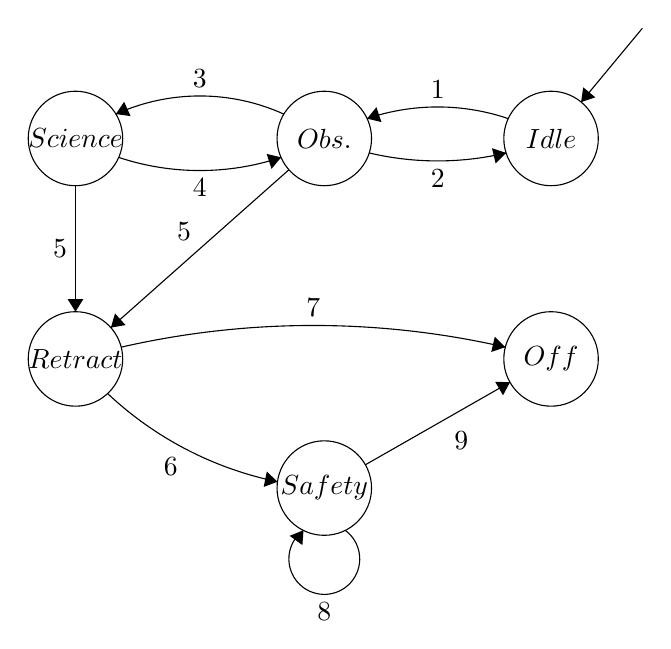
\begin{tikzpicture}[scale=0.2]
\tikzstyle{every node}+=[inner sep=0pt]
\draw [black] (46.2,-13.5) circle (3);
\draw (46.2,-13.5) node {$Idle$};
\draw [black] (31.8,-13.5) circle (3);
\draw (31.8,-13.5) node {$Obs.$};
\draw [black] (16,-13.5) circle (3);
\draw (16,-13.5) node {$Science$};
\draw [black] (16,-27.5) circle (3);
\draw (16,-27.5) node {$Retract$};
\draw [black] (46.2,-27.5) circle (3);
\draw (46.2,-27.5) node {$Off$};
\draw [black] (31.8,-35.7) circle (3);
\draw (31.8,-35.7) node {$Safety$};
\draw [black] (52,-6.5) -- (48.11,-11.19);
\fill [black] (48.11,-11.19) -- (49.01,-10.89) -- (48.24,-10.25);
\draw [black] (34.516,-12.239) arc (108.749:71.251:13.951);
\fill [black] (34.52,-12.24) -- (35.43,-12.46) -- (35.11,-11.51);
\draw (39,-11) node [above] {$1$};
\draw [black] (43.348,-14.419) arc (-76.68931:-103.31069:18.884);
\fill [black] (43.35,-14.42) -- (42.45,-14.12) -- (42.68,-15.09);
\draw (39,-15.43) node [below] {$2$};
\draw [black] (18.564,-11.955) arc (114.4174:65.5826:12.909);
\fill [black] (18.56,-11.95) -- (19.5,-12.08) -- (19.09,-11.17);
\draw (23.9,-10.3) node [above] {$3$};
\draw [black] (29.056,-14.702) arc (-71.60296:-108.39704:16.337);
\fill [black] (29.06,-14.7) -- (28.14,-14.48) -- (28.45,-15.43);
\draw (23.9,-16.04) node [below] {$4$};
\draw [black] (16,-16.5) -- (16,-24.5);
\fill [black] (16,-24.5) -- (16.5,-23.7) -- (15.5,-23.7);
\draw (15.5,-20.5) node [left] {$5$};
\draw [black] (29.55,-15.49) -- (18.25,-25.51);
\fill [black] (18.25,-25.51) -- (19.18,-25.35) -- (18.51,-24.61);
\draw (22.89,-20.01) node [above] {$5$};
\draw [black] (28.83,-35.296) arc (-101.59962:-133.25786:22.283);
\fill [black] (28.83,-35.3) -- (28.15,-34.65) -- (27.95,-35.63);
\draw (22.05,-33.75) node [below] {$6$};
\draw [black] (34.41,-34.22) -- (43.59,-28.98);
\fill [black] (43.59,-28.98) -- (42.65,-28.95) -- (43.15,-29.81);
\draw (40.5,-32.1) node [below] {$9$};
\draw [black] (33.123,-38.38) arc (54:-234:2.25);
\draw (31.8,-42.95) node [below] {$8$};
\fill [black] (30.48,-38.38) -- (29.6,-38.73) -- (30.41,-39.32);
\draw [black] (18.905,-26.751) arc (102.88102:77.11898:54.705);
\fill [black] (43.3,-26.75) -- (42.63,-26.09) -- (42.4,-27.06);
\draw (31.1,-24.87) node [above] {$7$};


\end{tikzpicture}
\end{center}



\begin{center}
Diagram of software states of operation and transition between states [2].

Transitions between states occur as numbered:

\begin{enumerate}
\item{\textbf{Appogee is reached.} The software shall activate when the power line goes to high at 28V. Observation mode shall be 
triggered when the \gls{OBC} turns on. Observation mode will collect a sweep of the payload with the camera. This mode will ensure that the 
camera is operational during the more crticial parts of the mission.}
\item{\textbf{Error: Return to Idle.} If an error is encountered in entering Observation mode, the software shall fallback to Idle 
mode and retry. An error may occur if the payload fails to deploy correctly or if the camera fails to turn on. The system shall send
a signal using the AVR interrupt library if the arm is not fully extended, as the arm is equipped with sensors to determine whether
it is extended or folded. If the camera fails to turn on, the system shall be notified as the telemetry line will be sending empty
data.}
\item{\textbf{Payload Assembly and Camera have been deployed.} The software shall enter Science mode once the payload assembly and arm
 have deployed and the camera has performed an observation sweep. Science mode will consist of the arm touching the sensors in 
 the payload canister, and collecting data via the telemetry line. The whole mode shall be captured with the camera.}
\item{\textbf{Error: Return to Observation} The software shall return to observation mode if any error occurs in Science mode. An error may occur in Science mode if the arm fails to operate correctly and must return to default position. An error may also occur if the camera stops working. The system shall know if the arm fails as a timer can keep track of the time between an arm movement request
and the arm actually completing the movement request. If too much time has elapsed between the request and the movement, the arm may
be stuck. If the telemetry line stops receiving data from the camera, then the camera has stopped working and the system shall be 
notified via an interrupt.}
\item{\textbf{Timer switches to end appogee period.} Once the time period for observation has ended, the timer line will go to low and trigger to Shutdown state. This state can be reached from either Observation or Science mode.}
\item{\textbf{Error: Shutdown not completed successfully.} If an error occurs in the shutdown sequence, the software shall enter Safety mode. An error that could occur is the arm failing to close, the Body failing to retract, or the \gls{OBC} not powering off. All 
these situations except for the \gls{OBC} not powering off are handled through Safety mode.}
\item{\textbf{Retry: Re-attempt to retract the arm.} Attempted to resolve any errors and retry retracting the arm.}
\item{\textbf{Accept: Shutdown correctly} If Shutdown occurs correctly, the arm should be closed, the Arm Assembly Body should be retracted, and the \gls{OBC} should be powered off. The arm will be have sensors to detect whether its closed or not, which can also
be used to know whether it has been retracted into the body. Once the system has determined that this criteria has been met, it
will power off.}
\item{\textbf{Error: Payload is still deployed.} The software shall remain in Safety mode until the payload is either retracted correctly, retracted fully with the arm in the open position, or ejected safely from the rocket. Safety mode shall first try to correctly retract the arm, then retract with the arm open, then repeat attempting ejection until the payload is ejected.}
\item{\textbf{Payload is Shutdown correctly.} If the payload is Shutdown through Safety mode, shutdown can be completed. In Safety mode, the payload was either shut down correctly, retracted fully into the can with the arm open, or the arm was expelled safely from the rocket. The shutdown sequence consists of the arm closing, the Body retracting, and the \gls{OBC} being powered off.}
\end{enumerate}
\end{center}

\subsubsubsection{Target Success Sensors}
\textbf{Author:} Amber Horvath
\label{subsec:tests}
\subsubsubsubsection{Requirement Overview}
The software shall know whether or not the arm succeeded in touching the targets generated, as described in subsection 2.1. The sensors
shall report back whether or not contact was made. This data can be used in post-mortem analysis to determine whether
certain targets were faulty or whether the range of motion on the arm was faulty.
\subsubsubsubsection{Solution Design}
The payload shall be equipped with pre-placed sensors that the arm shall make contact with. The arm shall have generated targets
as described in subsection 2.1. These coordinates shall be stored within the system and used as inputs for the function controlling
the arms' movements, with the target position being where the tip of the arm should be located. The arm shall exert force to touch
the sensor, and the sensor shall go high if contact is made. The sensors high or low signal shall be sent via the telemetry
line and written to our SD card. If the arm gets stuck during this process, it will enter Safety mode, as described in subsection 2.5. The telemetry data shall
later be visualized using Python's UI package, TK. 

\subsubsubsection{Telemetry}
\textbf{Author:} Michael Humphrey
\subsubsubsubsection{Requirement Overview}
The telemetry component shall report via telemetry all error codes and test results.

\subsubsubsubsection{Solution Design}
The telemetry component is responsible for collecting and sending data through the
telemetry ports on the \gls{payload}.

This component shall not be responsible for transmitting data generated from the
temperature sensors.
The temperature sensors will be wired directly to an analog telemetry port,
bypassing the \gls{OBC} altogether.

For each test the software successfully completes (see \hyperref[subsec:tests]{subsection 
\ref*{subsec:tests},  Target Success Sensors}) this component shall output a code
representing the test number to the telemetry port.
There shall be two tests; one for each touch point on the \gls{payload}.
The tests shall be designed as a joint effort between the Hephaestus Structures,
Robotics, Electrical, and Software teams.

The output shall be encoded as a four character \gls{binstring} and transmitted
simultaneously via a four parallel port pins.
The \gls{binstring} shall be transmitted at a rate of no more than 5,000 Hz.
There shall be a delay of no less than .2 milliseconds between transmissions
of codes.
When no code is being actively transmitted, the telemetry shall output a code
of `0000' to the telemetry pins.

In addition to transmitting codes via the telemetry lines, the software shall also
store a log file with timestamps on an onboard SD card.
The log file shall consist of a series of lines of text, consisting of a timestamp
and a description.
The timestamp shall be the number of tenths of milliseconds since the \gls{OBC}
powered on.
The description shall be a sequence of \gls{ASCII} characters of arbitrary length,
and terminated with a carriage return character.

\subsubsubsection{Video Handling}
\textbf{Author:} Michael Humphrey
\subsubsubsubsection{Requirement Overview}
Video footage of the \gls{payload}'s operations shall be recorded and saved to the
SD card.

\subsubsubsubsection{Solution Design}
The Hephaestus Electrical Engineering team shall design the payload such that the 
camera will power on and off at the appropriate times, as well as save footage to
the SD card. 

\subsubsubsection{Data Visualization and Processing}
\textbf{Author:} Michael Humphrey
\subsubsubsubsection{Requirement Overview}
The data visualization and processing component shall provide visualizations
for the collected data.
This component shall be able to show whether the mission success criteria have
been met or not.
If the mission success criteria have not been met, this component shall show how
and why they have not been met.

\subsubsubsubsection{Solution Design}
The component shall have a \gls{gui} written in Tkinter with graphs generated by
\gls{matplotlib}.
The \gls{gui} shall consist of two graphs, a table, and a timeline.
Each graph shall be a \gls{plot} with analog data collected from each of two temperature sensors.
The data from the temperature sensors shall be graphed with respect to time from
\gls{apogee} and actual temperature, if such a value can be determined.
In the absence of a method to reliably determine actual temperature from the raw
sensor data, then the data shall be graphed with respect to the raw value received
from the sensor, with the graph scaled such that the lowest value recorded shall be
the minimum y value, and the highest recorded value recorded shall be the maximum y value.
The user shall be able to scale the graphs to view portions of the data as they see fit.
The table shall consist of the name of each of a series of tests,
the result of that respective test, and the time that test was completed.
A result shall be either ``passed'', ``failed'', or ``not completed''.
A result of ``passed'' shall be colored in green.
A result of ``failed'' shall be colored in red.
A result of ``not completed'' shall be colored in yellow.
If the result of a test is ``not completed'', then the time of completion for that test
may be omitted.
There shall be two total tests.
The tests shall be for if the \gls{payload} can successfully touch each touch point sensor.
The tests shall be designed as a joint effort between the Hephaestus Structures,
Robotics, Electrical, and Software teams.
The timeline shall be a visualization with time on the y axis, with significant events
marked at various positions along the axis, according to when that event happened.


\subsubsection{Conclusion}
This concludes the design of our project. Further questions or concerns can be addressed to the authors of this document.
This document may be subject to changes in the future as more design constraints are found, or designs are found to not work the way



\subsection{Changes Since Original Design Document}
\input{./parts/ChangesinDesign.tex}

\section{Technical Review Document}
\subsection{Original Technical Review Document}
\subsection{Introduction}
\subsubsection{Document Overview}
This is the Technical Review And Implementation Plan for the Hephaestus project.
This document shall investigate possible methods of implementing our project software requirements.
The nine general requirements investigated below were identified as project requirements in our Requirements document.
This document will focus on the "how" of our requirements implementation.
\subsubsection{Role Breakdown}
Each CS Senior Design team member shall be responsible for ensuring the completion of the three items
from the requirements document that are assigned to them below.
\subsubsubsection{Helena Bales}
\begin{enumerate}
\item{Target Generation}
\item{Arm Movement}
\item{Arm Position Tracking}
\end{enumerate}
\subsubsubsection{Amber Horvath}
\begin{enumerate}
\item{Emergency Payload Expulsion}
\item{Program Modes of Operation}
\item{Target Success Sensors}
\end{enumerate}
\subsubsubsection{Michael Humphrey}
\begin{enumerate}
\item{Telemetry}
\item{Video Camera}
\item{Data Visualization and Processing}
\end{enumerate}

\subsection{Technologies}
\subsubsection{Target Generation}
\subsubsubsection{Requirement Overview}
The software shall generate points to be used in testing the Hephaestus arm.
The points will constitute the total test of the arm, and should therefore include points
representative of standard and edge cases.
These points shall be used as targets for the arm body.
\subsubsubsection{Proposed Solutions}
\begin{enumerate}
\item{
\textbf{The points shall be generated in 3-D polar form}, including an angle from normal, a radius, 
and a height. 
The angle shall be in the range of 0 and 359 degrees.
An angle of zero degrees shall be in the direction of payload deployment.
The radius shall be the distance from the arm's attachment to the base to the generated point.
The height of the point, for the purpose of target generation, shall be constant.
However the points will always be stored in a triple of angle from normal (\(\theta\)), radius (\(r\)), and height (\(h\)).
}
\item{
\textbf{The points shall be generated in 3-D Cartesian form}, including \(x\) position to the right 
or left of the \(y-axis\), the \(y\) position above or below the \(x-axis\), and the height, \(h\), 
above the \(xy-plane\).
Let the \(y-axis\) be the direction that the payload deploys from the can.
Let the \(x-axis\) be the perpendicular to the \(y-axis\) at the point where the arm is mounted 
to the rotating plate. 
Let \(h\) be the height above the \(xy-plane\), where the arm is attached to the rotating plate.
}
\item{
\textbf{The points shall be generated in 2-D Polar coordinates}, where the implementation is the 
same as described in the 3-D Polar coordinate section, with the exception of \(h\).
In this case, there shall be no \(h\).
The position can be represented in 2-D Polar coordinates on the plane of the base plate.
For the purpose of compatibility with the position of the arm, the height could be assumed to be 0.
}
\end{enumerate}

\subsubsection{Arm Movement}
\subsubsubsection{Requirement Overview}
The software shall control the movement of the arm body assembly. 
The position of the tip of the arm shall be tracked in the coordinate notation described in section 2.2 above.
The software shall rotate the arm body assembly in a full 360 degrees.
The software shall additionally control the movement the height of the arm body assembly.
The arm should descend and touch the baseplate of the payload at any rotation.
\subsubsubsection{Proposed Solutions}
\begin{enumerate}
\item{
\textbf{The movement of the arm shall be generated by a custom system where the movement of the arm is 
generated based on the current position and the starting position.} 
The position of the tip of the arm shall be stored as decided from the list of solutions above. 
In the case of the selection of solution 3, the position will have an added height. 
The position shall be denoted as point \(p\) and shall be the location of the tip of the arm.
The arm shall generate a series of commands for the motors to perform to go from \(p\) to the target, 
\(t_{n}\) where \(t_{n}\) is the n-th target.
}

\item{
\textbf{The movement of the arm shall be generated by a custom system where the movement of the arm is 
generated based on the current position and the starting position.} 
The position of the tip of the arm shall be stored as decided from the list of solutions above. 
In the case of the selection of solution 3, the position will have an added height. 
The position shall be denoted as point \(p\) and shall be the location of the tip of the arm.
The arm shall generate a series of commands for the motors to perform to go from \(p\) to the target, 
\(t_{n}\) where \(t_{n}\) is the n-th target.
The movement of the arm shall be constrained by the heights of the arm so that it will not collide with 
the top or base plates.
}

\item{
\textbf{The movement of the arm shall be accomplished by turning the arm to the correct \(\theta\), then correct radius, then correct height.}
The rotating base plate will be responsible for turning the arm to the correct \(\theta\) value.
The motors, labeled \(m1\), and \(m2\), shall be responsible for moving the arm to the correct radius and
 height. The position of the arm, \(p\), and the target position \(t_{n}\), shall be stored in the 
manner described in the section titled Arm Position Tracking.
}

\item{
\textbf{The movement of the arm shall follow a path through a 4-degree of freedom (dof) configuration
space.} The path of the arm shall be generated using the A* pathfinding algorithm. The configuration 
		space shall be in \(\rm I\!R^4\). Valid points in the configuration space will be represented by a 0, 
while invalid points will be represented by a 1. A point in the configuration space represents the 
angles at which the four arm actuators are bent. In this way, the position of the arm can be uniquely
 represented. An area in the configuration space maps to a single point in real space.

In order to move from one point to the next, a path will be generated using A* from the starting position to the final position. The final position will be converted from Real Space to the C-Space using 
Inverse Kinematics. Once the path has been generated, the arm will be moved through the path from the 
initial configuration through the list of configurations given by the path. In moving from one 
configuration to the next, the motors will be rotated to the new configuration starting at the base of
the arm towards the tip of the arm.
}
\end{enumerate}

\begin{center}
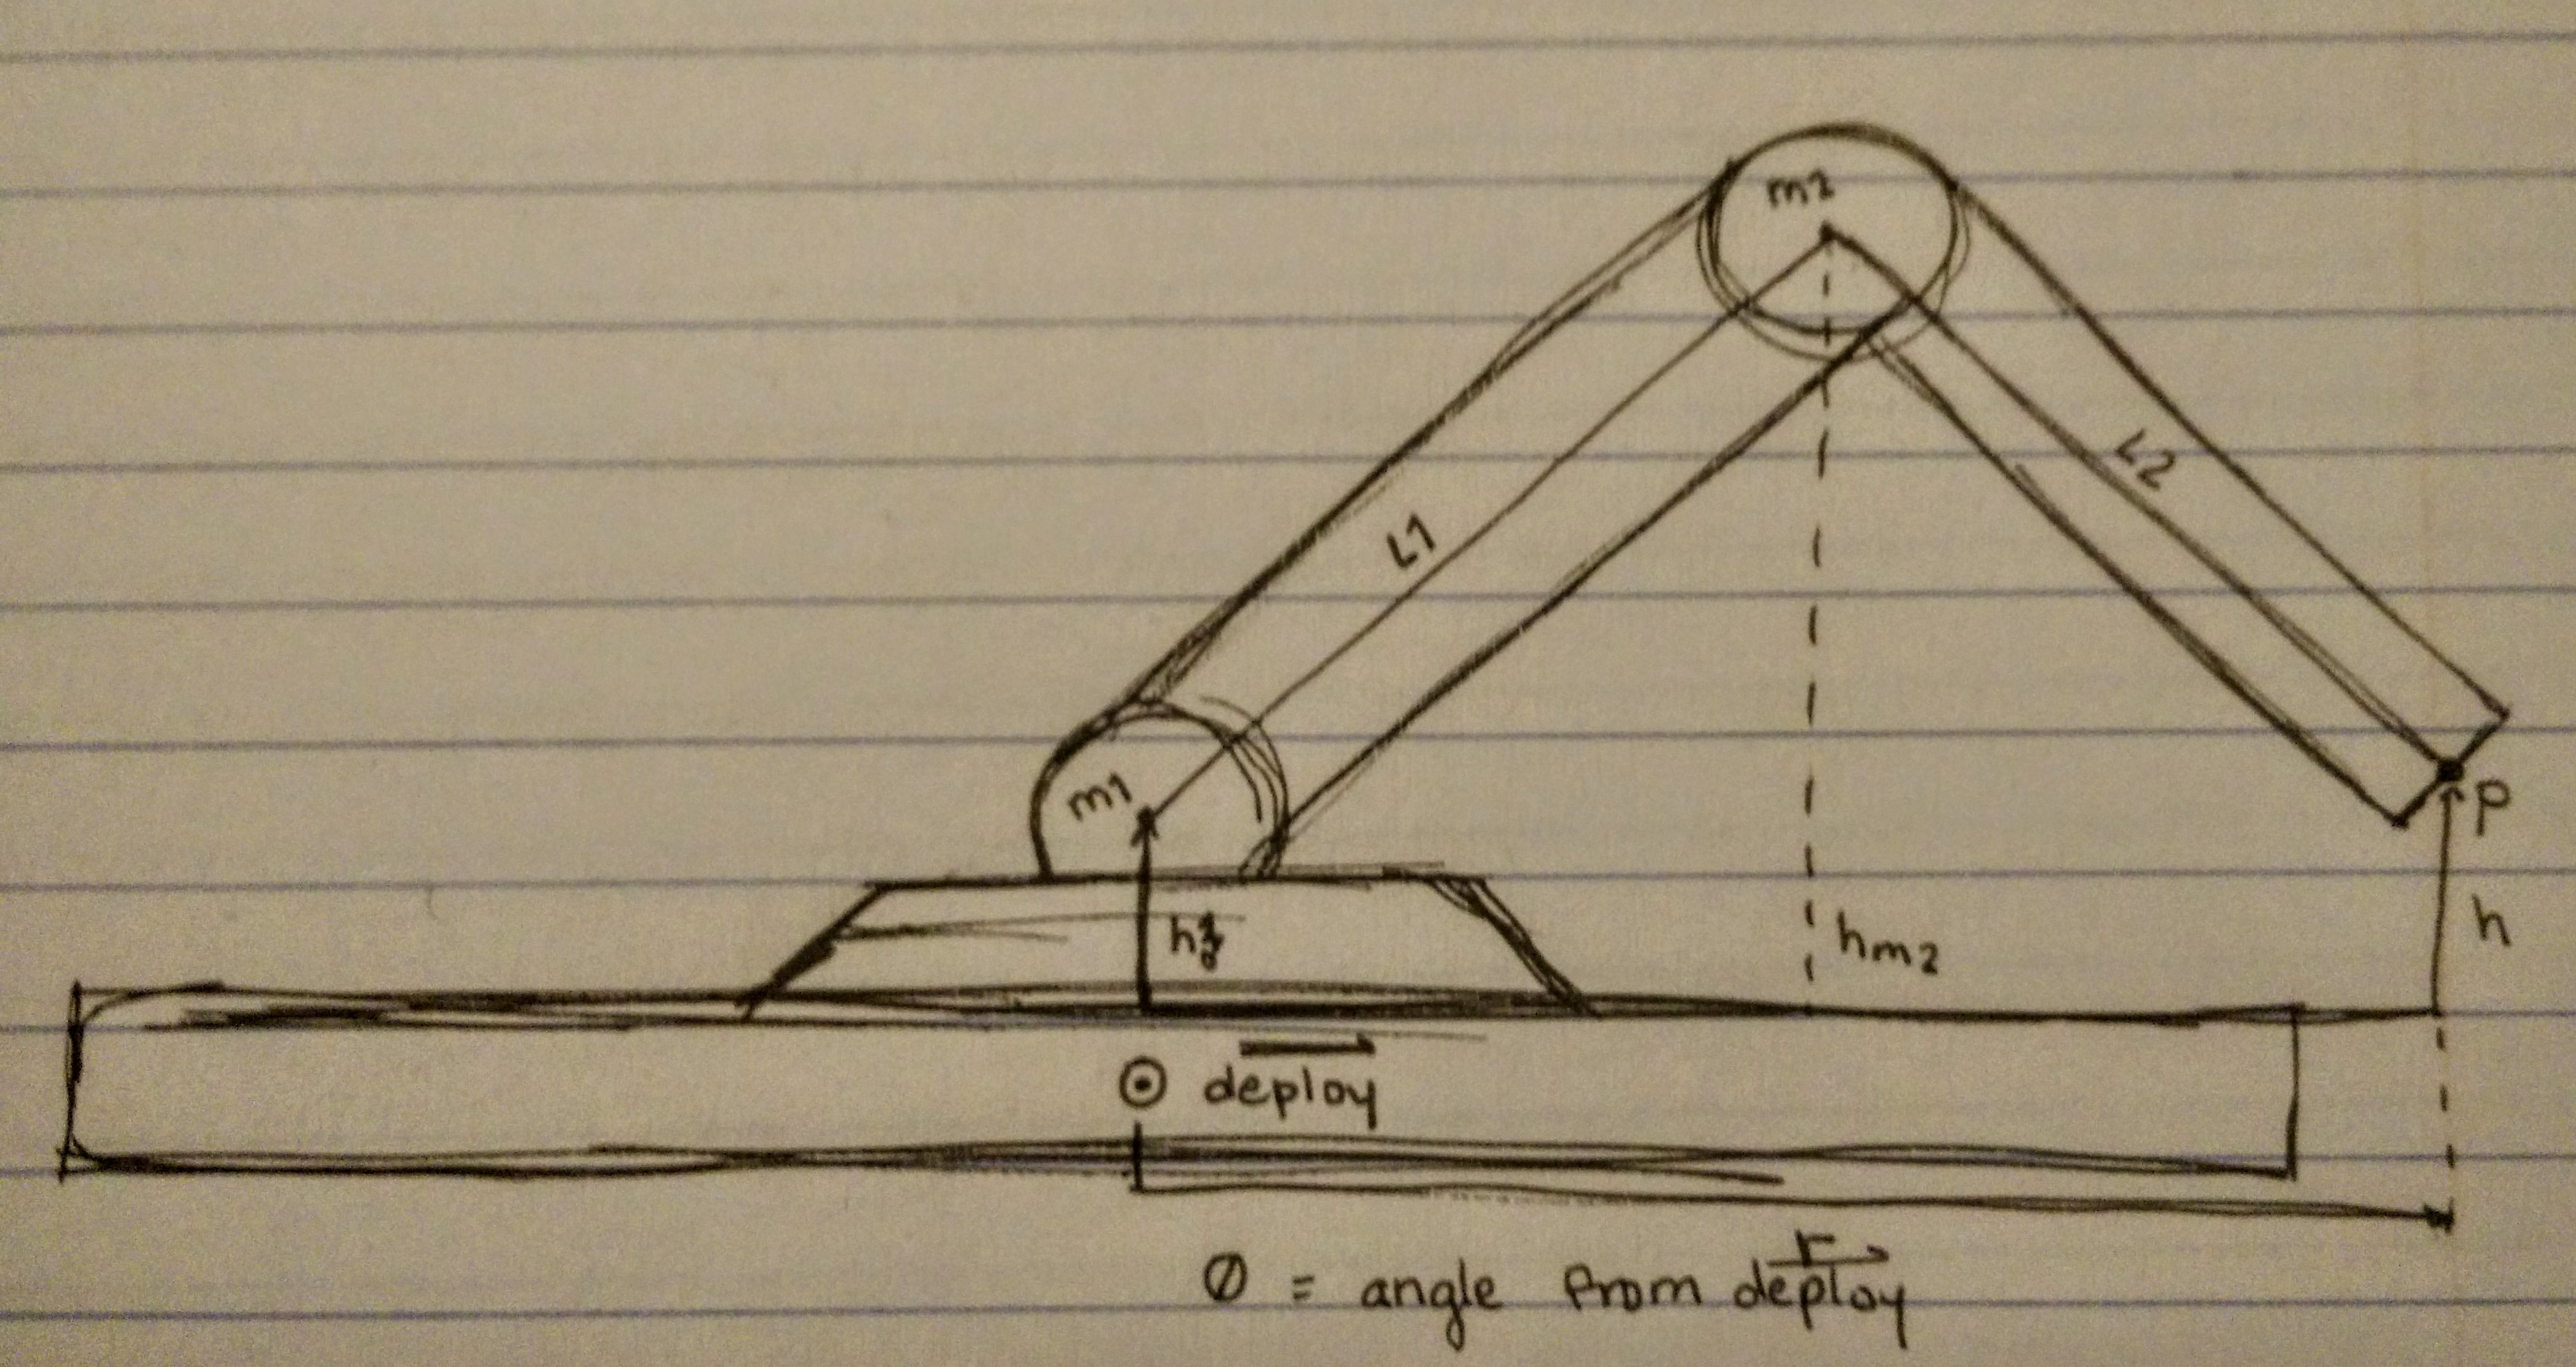
\includegraphics[width=\textwidth]{./images/armDiagram}
\textbf{Figure 1} -- Arm Movement Design
\end{center}

\subsubsection{Arm Position Tracking}
\subsubsubsection{Requirement Overview}
The position of the arm shall be tracked using the same coordinate system described in the Target Generation requirement.
The position of the arm shall be calculated using the known start position and the rotation of the motors.
The starting position shall be known due to a calibration point that will allow for a reset at any time.
Resetting in this way will allow for flexibility between resetting for maximum operation time with only tolerably small error defined by the Non Functional Requirements.
\subsubsubsection{Proposed Solutions}
\begin{enumerate}
\item{
\textbf{The position of the arm shall be tracked using the motor movement.}
The initial position of the arm shall be defined in advance, and a sensor will be placed at that location. 
From there, the position will be tracked from the movement of the motors.
The arm will recalibrate by returning to the initial position in order for the error to not increase over
 time.
The position of the arm shall be denoted \(p\), the location of the tip of the arm.
This shall be the only position tracked.
}
\item{
\textbf{The position of the arm shall be tracked using the motor movement to calculate \(p\) and 
\(p_{m2}\).}
The initial position of the arm shall be defined in advance, and a sensor will be placed at that location. 
From there, the position will be tracked from the movement of the motors.
The arm will recalibrate by returning to the initial position in order for the error to not increase over
 time.
The position of the arm shall be denoted \(p\), the location of the tip of the arm.
From the coordinate \(p\), the location of \(p_{m2}\), the center of the middle joint of the arm, will be
 calculated. The height of \(p_{m2}\) will be calculated from the triangle made of the two arm sections, 
L1 and L2, and the radius of point \(p\). From there the radius of the point \(p_{m2}\) can be calculated
 using the triangle of L1, \(h_{m2}\) and the radius of m2. Finally, the \(\sigma\) of \(p_{m2}\) shall 
be the same as that of \(p\).
Using this method will allow for the extra condition that point \(p_{m2}\) should never exceed the height
 of the can.
}
\item{
\textbf{The position of the arm shall be tracked using the motor movement to calculate \(p\), with a
 limit on the height of the arm.}
The initial position of the arm shall be defined in advance, and a sensor will be placed at that location. 
From there, the position will be tracked from the movement of the motors.
The arm will recalibrate by returning to the initial position in order for the error to not increase over
 time.
The position of the arm shall be denoted \(p\), the location of the tip of the arm.
This will be the only point tracked, however the values of \(p\) shall be restricted such that the 
height of the arm never exceeds the height of our half can.
}


\end{enumerate}

\subsubsection{Emergency Payload Expulsion}
\subsubsubsection{Requirement Overview}
The software shall eject the arm upon system failure. 
System failure in this case is defined as the arm becoming lodged or stuck in a state where it is unable to retract.
The software will enter Safety mode (defined in section 2.5.2) and attempt to retract the arm. If it is unable to complete this step,
 the system will continue attempting to eject the arm until ejection is completed
\subsubsubsection{Proposed Solutions}
\begin{enumerate}
\item{
\textbf{The software accepts a signal sent from the Shutdown state to the Safety state}
Upon entering the Shutdown state, the system should succeed in closing the arm, the Arm Assembly Body should be retracted, 
and the OBC should be powered off. If any of these conditions are not met, a signal should be sent, resulting in a change of state
from the Shutdown state to the Safety state, where the arm can be ejected.
}
\item{
	\textbf{The software sends a signal to enter Safety state upon any failure to complete an arm-movement task}
A timer should be implemented to detect whether a certain amount of time has elapsed between the last arm movement and the last 
request for an arm movement. If arm movement requests are not being met by arm movements, and the system stalls past a certain amount 
of time, the system should send a signal to enter the Safety state so that the arm can be ejected, as it is most likely caught
in a bad extended position.
}
\item{
	\textbf{The software shall notify via telemetry that ejection was required}
In the post-mortem analysis, we will want to know whether an ejection was necessary and what caused the bad state. The system
shall, upon receiving a signal that ejection is required, send a log description of the current coordinates of the arm, the time 
elapsed since last arm movement request, and what state the system was in prior to being sent to the Safety state.
}
\end{enumerate}
\subsubsection{Program Modes of Operation}
\subsubsubsection{Requirement Overview}
The software shall have the Modes of Operation necessary to insure the mission success.
The software shall first deploy the payload, then the arm. Next the software shall activate the 
camera and perform a video sweep. The software shall then perform the science experiment.
If the experiment fails, it shall return to observation mode.
If observation mode fails, it shall return to idle.
Once the experiment time has been exhausted, the payload shall shut down.
If it shuts down correctly, everything will poweroff. If not, the payload shall attempt to retract 
again, or expel the payload from the rocket.
\subsubsubsection{Proposed Solutions}

\begin{center}
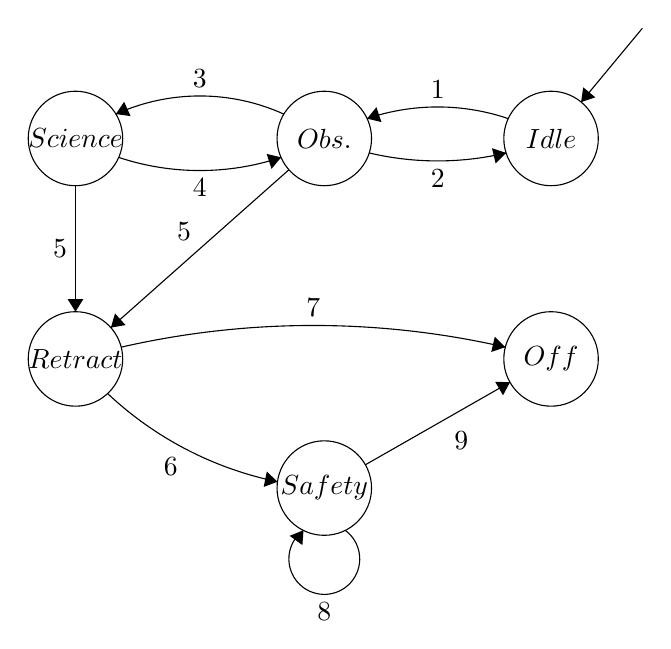
\begin{tikzpicture}[scale=0.2]
\tikzstyle{every node}+=[inner sep=0pt]
\draw [black] (46.2,-13.5) circle (3);
\draw (46.2,-13.5) node {$Idle$};
\draw [black] (31.8,-13.5) circle (3);
\draw (31.8,-13.5) node {$Obs.$};
\draw [black] (16,-13.5) circle (3);
\draw (16,-13.5) node {$Science$};
\draw [black] (16,-27.5) circle (3);
\draw (16,-27.5) node {$Retract$};
\draw [black] (46.2,-27.5) circle (3);
\draw (46.2,-27.5) node {$Off$};
\draw [black] (31.8,-35.7) circle (3);
\draw (31.8,-35.7) node {$Safety$};
\draw [black] (52,-6.5) -- (48.11,-11.19);
\fill [black] (48.11,-11.19) -- (49.01,-10.89) -- (48.24,-10.25);
\draw [black] (34.516,-12.239) arc (108.749:71.251:13.951);
\fill [black] (34.52,-12.24) -- (35.43,-12.46) -- (35.11,-11.51);
\draw (39,-11) node [above] {$1$};
\draw [black] (43.348,-14.419) arc (-76.68931:-103.31069:18.884);
\fill [black] (43.35,-14.42) -- (42.45,-14.12) -- (42.68,-15.09);
\draw (39,-15.43) node [below] {$2$};
\draw [black] (18.564,-11.955) arc (114.4174:65.5826:12.909);
\fill [black] (18.56,-11.95) -- (19.5,-12.08) -- (19.09,-11.17);
\draw (23.9,-10.3) node [above] {$3$};
\draw [black] (29.056,-14.702) arc (-71.60296:-108.39704:16.337);
\fill [black] (29.06,-14.7) -- (28.14,-14.48) -- (28.45,-15.43);
\draw (23.9,-16.04) node [below] {$4$};
\draw [black] (16,-16.5) -- (16,-24.5);
\fill [black] (16,-24.5) -- (16.5,-23.7) -- (15.5,-23.7);
\draw (15.5,-20.5) node [left] {$5$};
\draw [black] (29.55,-15.49) -- (18.25,-25.51);
\fill [black] (18.25,-25.51) -- (19.18,-25.35) -- (18.51,-24.61);
\draw (22.89,-20.01) node [above] {$5$};
\draw [black] (28.83,-35.296) arc (-101.59962:-133.25786:22.283);
\fill [black] (28.83,-35.3) -- (28.15,-34.65) -- (27.95,-35.63);
\draw (22.05,-33.75) node [below] {$6$};
\draw [black] (34.41,-34.22) -- (43.59,-28.98);
\fill [black] (43.59,-28.98) -- (42.65,-28.95) -- (43.15,-29.81);
\draw (40.5,-32.1) node [below] {$9$};
\draw [black] (33.123,-38.38) arc (54:-234:2.25);
\draw (31.8,-42.95) node [below] {$8$};
\fill [black] (30.48,-38.38) -- (29.6,-38.73) -- (30.41,-39.32);
\draw [black] (18.905,-26.751) arc (102.88102:77.11898:54.705);
\fill [black] (43.3,-26.75) -- (42.63,-26.09) -- (42.4,-27.06);
\draw (31.1,-24.87) node [above] {$7$};


\end{tikzpicture}
\end{center}



\begin{center}
Diagram of software states of operation and transition between states [2].

Transitions between states occur as numbered:

\begin{enumerate}
\item{\textbf{Appogee is reached.} The software shall activate when the power line goes to high at 28V. Observation mode shall be triggered when the OBC turns on.}
\item{\textbf{Error: Return to Idle.} If an error is encountered in entering Observation mode, the software shall fallback to Idle mode and retry. An error may occur if the payload fails to deploy correctly or if the camera fails to turn on.}
\item{\textbf{Payload Assembly and Camera have been deployed.} The software shall enter science mode once the payload assembly and arm have deployed and the camera has performed an observation sweep.}
\item{\textbf{Error: Return to Observation} The software shall return to observation mode if any error occurs in Science mode. An error may occur in Science mode if the arm fails to operate correctly and must return to default position. An error may also occur if the camera stops working.}
\item{\textbf{Timer switches to end appogee period.} Once the time period for observation has ended, the timer line will go to low and trigger to Shutdown state. This state can be reached from either Observation or Science mode.}
\item{\textbf{Accept: Shutdown correctly} If Shutdown occurs correctly, the arm should be closed, the Arm Assembly Body should be retracted, and the OBC should be powered off.}
\item{\textbf{Error: Shutdown not completed successfully.} If an error occurs in the shutdown sequence, the software shall enter Safety mode.}
\item{\textbf{Payload is Shutdown correctly.} If the payload is Shutdown through Safety mode, shutdown can be completed. In Safety mode the payload was either shut down correctly, retracted fully into the can with the arm open, or the arm was expelled safely from the rocket.}
\item{\textbf{Error: Shutdown not completed successfully.} If an error occurs in the shutdown sequence, the software shall enter Safety mode.}
\item{\textbf{Payload is Shutdown correctly.} If the payload is Shutdown through Safety mode, shutdown can be completed. In Safety mode the payload was either shut down correctly, retracted fully into the can with the arm open, or the arm was expelled safely from the rocket.}
\item{\textbf{Error: Payload is still deployed.} The software shall remain in Safety mode until the payload is either retracted correctly, retracted fully with the arm in the open position, or ejected safely from the rocket. Safety mode shall first try to correctly retract the arm, then retract with the arm open, then repeat attempting ejection until the payload is ejected.}
\end{enumerate}
\end{center}

\subsubsection{Target Success Sensors}
\subsubsubsection{Requirement Overview}
The software shall know whether or not the arm succeeded in touching the targets generated, as described in section 2.1. The sensors
shall report back whether or not contact was made. This data can be used in post-mortem analysis to determine whether
certain targets were faulty or whether the range of motion on the arm was faulty.
\subsubsubsection{Proposed Solutions}
\begin{enumerate}
\item{
	\textbf{The software shall store the coordinates produced during the target generation stage and compare with the targets actually
	reported after the arm moves}
The software shall have generated a coordinate (the form yet to be determined) that is sent to the arm to move to that specificied 
location. Post-movement, the arm can keep determine its movement using the motor and the sensor described in section 2.3. A check for
equality can be performed between these two points to determine whether the points are equivalent or not. If they are equivalent, the
movement was successful and resulted in the target being touched. If the equivalency fails, then the arm did not meet its target
and should be set back to a pre-determined starting position to prevent further target points from being influenced by the margin
of error. Both a successful target touch and a failed target touch should be stored so as to keep track of the ratio between successful
and unsuccessful trials.
}
\item{
	\textbf{The software shall evaluate a delta between the point generated and the actual point reported}
A delta can be determined between the arm movement and the difference between that position and the calibration point, where the 
calibration point is a stored value. If the delta is 0, then the point generated was correct. If not, then the arm should be set 
back to a stored location to prevent the margin of error influencing further target generation and touches. Both a successful 
target touch and a failed target touch should be stored so as to keep track of the ratio between successful
and unsuccessful trials.
}
\item{
	\textbf{The stored video and telemetry data shall work as an oracle when evaluating our success sensors}
	This is the least reliable of our methods, as relying on the video capture is risky, along with the less rigorous methodology.
	However, if all else fails, we can comb over the telemetry data and the stored video capture to determine whether or not the arm
	succeeded or failed in touching the generated targets by watching the video and comparing it to the telemetry data. We would be 
	looking for instances where the sensor data captured via telemetry matches with video footage of the arm extending and touching
	a generated point to see whether the data matches up with the video feed.
}
\end{enumerate}
\subsubsection{Telemetry}
\subsubsubsection{Requirement Overview}
The software shall report via telemetry all sensor data.

The criteria that these technologies will be evaluated on is:
\begin{itemize}
\item \textbf{Ease of use.}
The chosen solution should let the developers focus on writing code and not encoding data for telemetry transmission.
Ideally, sending data through one of the telemetry ports should be no more than one line of code. 
\item \textbf{Reliability.}
The chosen solution should be able to relay 100\% of transmitted data to the ground station without corrupting or losing any of it.
\item \textbf{Documentation.}
The chosen solution should be well documented.
The developers should be able to quickly and easily locate supporting documentation for using the technology.
\item \textbf{Compatibility.}
The chosen solution should be compatible with the software and hardware of the \gls{payload}.
\end{itemize}

\subsubsubsection{Proposed Solutions}
The three options being considered for transmitting telemetry are
\begin{enumerate}
\item{
\textbf{A custom-built solution for our own needs}.
The custom-built solution is the least appealing. It would require the most amount of work to develop and maintain by the developers.
The advantage of a custom-built solution is that it can be tailored to the requirements of our system, making it extremely to use.
However, the benefit is offset by the huge amount of work upfront it would require to develop and test the solution.
Since the developers would be coding up this solution themselves, it would require a lot of testing to ensure a reliable solution.
The hand-written test cases cannot guarantee the reliability of the solution, 
especially given the relative inexperience of the developers with writing code for this platform.
Therefore one can expect to have relatively unreliable code and encounter lots of bugs.
Compatibility would not be a problem with this solution because the code would be custom-made for the hardware.
However, documentation would be non-existent because the developers would be writing the code themselves.
The only documentation that would be relevant would be from other projects that have written telemetry code for spacecraft.
However, most of that documentation would be internal to the organizations building the spacecraft,
most likely wouldn't be helpful.
}

\item{
\textbf{Open MCT developed by NASA for space-specific missions}
Open MCT is a mission control framework developed and used by NASA.
Because of the many requirements by NASA, Open MCT is a vast and complicated framework.
It is incredibly complicated and requires a lot of code in order to do simple tasks.
However, because it is supported by NASA, it is highly reliable for space applications.
There is lots of documentation on the Open MCT website for developers.
However, it appears that Open MCT does not support telemetry from the spacecraft.
It does, however, support data visualization out of the box. (See section 2.9)
}

\item{
\textbf{PSAS Packet Serializer developed by \gls{psas}.}
PSAS Packet Serializer is a student aerospace engineering project developed by \gls{psas} at \gls{psu}. 
The project seeks to create a standard way to encode data for telemetry transmission between various components
and the ground station.
This solution would be very easy to use because of its simple interface.
Only one line is required to both encode and decode data.
This solution is also extremely reliable since it has been used in several flights by the \gls{psu} team.
The solution is also well-documented.
There is an entire website dedicated to documenting the simple \gls{api}.
However, the major problem with this solution is compatibility.
The solution is implemented in Python, whereas the code for the \gls{payload} is restricted to C.
It is not feasible to run the Python implementation on the microcontroller in C,
but it may be possible to \gls{port} the code to C.
This would require a lot of unpleasant work on the developers' part.
The goal for this technology is to let the developers quickly and easily relay data to the ground station.
}
\end{enumerate}
Despite many disadvantages, the best option for now appears to be creating a
custom-built telemetry solution due to compatibility issues with the other solutions.

\subsubsection{Video Handling}
\subsubsubsection{Requirement Overview}
The software shall be responsible for controlling the camera output.

The criteria that these technologies will be evaluated on is:
\begin{itemize}
\item \textbf{Reliability.}
The solution should guarantee that video footage is permanently recorded.

\item \textbf{Ease of use.}
The solution should be easy to implement and use.
\end{itemize}

\subsubsubsection{Proposed Solutions}
The three options being considered for controlling the camera are:
\begin{enumerate}
\item{
\textbf{Enabling and disabling a third-party camera.}
This solution involves turning on and off a self-contained third-party camera.
Defining what the camera will be is outside of the scope of the Hephaestus software team.
The camera used will be decided by the Hephaestus electrical and robotics teams
based on their design requirements.
Currently, a GoPro is the most likely to be used for the camera.
Self-contained shall be defined as a product that can start, stop, and store video
footage without any outside input.
The software shall enable video recording at the beginning of the demonstration,
and stop video recording at the end.
}

\item{
\textbf{Enabling/disabling an on-board camera, and storing video output.}
This solution involves turning on and off a video camera, as well as processing and storing the video output.
Defining what the camera will be is outside of the scope of the Hephaestus software team.
The camera used will be decided by the Hephaestus electrical and robotics teams
based on their design requirements.
The software shall start video recording at the beginning of the demonstration,
and stop video recording at the end.
Additionally, the software shall process the output of the video camera and store
it in a location so that it can be recovered after the rocket returns to earth.
}

\item{
\textbf{Enabling/disabling an on-board camera, and transmitting video output through telemetry ports.}
This solution involves turning on and off a video camera, as well as processing and transmitting the video output though the telemetry ports.
Defining what the camera will be is outside of the scope of the Hephaestus software team.
The camera used will be decided by the Hephaestus electrical and robotics teams
based on their design requirements.
The software shall start video recording at the beginning of the demonstration,
and stop video recording at the end.
Additionally, the software shall process the output of the video camera and transmit
it through the telemetry ports to the ground station.
In the event of the rocket not being recovered, the video feed can still be kept
from the telemetry playback.
}
\end{enumerate}

The recommended solution for this technology is enabling and disabling a third-party camera.

\subsubsection{Data Visualization and Processing}
\subsubsubsection{Requirement Overview}
After the mission completes, the software shall provide visualizations for the collected data.
The software shall be able to show whether the mission success criteria have been met or not.
If the mission success criteria have not been met, the software shall show how and
why they have not been met.

The criteria that these technologies will be evaluated on is:
\begin{itemize}
\item \textbf{Cross-platform compatibility.}
The chosen solution should be able to run across any of the major computing platforms.

\item \textbf{Range and variety of visualization methods.}
The chosen solution should have a large variety of different visualization methods.

\item \textbf{Documentation.}
The chosen solution should be well documented.
The developers should be able to quickly and easily locate supporting documentation for using the technology.

\item \textbf{Developer proficiency.}
The majority of developers should be able to comfortably develop the visualizations
without needing to learn any new technologies.
\end{itemize}

\subsubsubsection{Proposed Solutions}
The three options being considered for visualizing the data are:
\begin{enumerate}
\item{
\textbf{Matplotlib.}
Matplotlib is a Python plotting and graphing library.
Matplotlib is written in Python, and will therefore run on all platforms that Python supports.
Matplotlib supports both 2d and 3d graphics, and can render dozens of different
types of graphs.
Since Matplotlib is used and supported by thousands of developers, there is ample
documentation for all aspects of the library.
All core developers for the Hephaestus mission are familiar with Python.
}

\item{
\textbf{Vis.js.}
Vis.js is a Javascript library for constructing graphs in a browser.
Since it is rendered in a browser, it is accessible on all platforms with a web browser
that runs Javascript.
Vis.js lists 20 different 2d graphs on its website and 13 different 3d graphs, as well
as other graphs including timelines and networks. 
Vis.js has less documentation for it on its website, and because it's a smaller library
there are less third-party resources for learning it online.
However, there is enough documentation to start using it on its website.
The \gls{api} is easy enough that there should not be any significant challenges
because of the lack of documentation.
Only about half of the Hephaestus development team is familiar with Javascript,
so that may be an obstacle going forward if this solution is used.
}

\item{
\textbf{Lighting.}
Lighting provides a unique and flexible way to create graphs.
Instead of using a library to render graphs, Lighting uses a web server to
render the graphs.
Developers can request a server to render a graph, and then retrieve it either via
a RESTful web \gls{api} or through one of several client libraries.
Developers can either opt to run their own server, or use one of several public
servers Lightning has provided for free.
Because Lighting doesn't restrict what programming language you can use to
create charts and graphs, the developers are free to choose whatever language
they are most proficient in.
Lighting also provides the ultimate level of cross-compatibility among platforms
because it is completely platform agnostic.
Since it runs in a server by itself, it can be accessed by any platform with a TCP/IP stack.
Lighting lists 15 different graphs it can render by default; with the potential to add
many more.
Lighting can be extended to support more kinds of graphs though \gls{npm} modules.
Lightning provides a variety of documentation sources on its website.
There isn't an overwhelming abundance of documentation, but it appears to be
enough to successfully start developing charts and graphs using it.
}
\end{enumerate}

The recommended solution for this technology is Lightning.

\subsection{Conclusion}
The Hephaestus RockSat-X Payload will continue with the implementation of one of the listed possible 
solutions to each of the nine requirements outlined in this document.
The development of the software will begin through the end of Fall term of 2016 and continue during 
the Winter 2017 term. Once we have obtained the hardware for the arm, we shall begin development of the 
arm control software, the video recording, and the payload behavior for the duration of the flight. This 
development will be followed by thourough testing, which will be described in future documents.




\subsection{Changes Since Original Technical Review Document}
We did not make any changes to our tech review document.

\section{Weekly Blog Posts}
\subsection{Fall 2016}
\subsubsection{Week 3}
\subsubsubsection{Helena Bales}
\textbf{Progress} \\
This week I made significant strides in the design of our project. I wrote part of the Project Definition assignment. I started the Project Description with a description of the problem, broken down into the requirements of the RockSat-X program and the payload that we decided on for the project. In order for our senior design project to be successful, we have to build the payload, meet the RockSat-X project requirements (such as testing, documentation, and design reviews), and meet the capstone class requirements. Our payload idea is a mechanical arm, and as a project it is capable of meeting all the requirements.

While the Project Definition document met our capstone class requirements for the week, there were also RockSat-X requirements to be met this week. The RockSat-X CoDR (Conceptual Design Review) was this week. As a large group (including two teams of ME's, one team of EE's, and the CS team) we developed the CoDR powerpoint that was presented yesterday to RockSat-X. This document included all of our conceptual payload designs thus far, and was our first time presenting our designs to the RockSat-X group. Following that presentation, in order to meet the RockSat-X requirements, we took a group photo.

In addition to the RockSat-X requirements and the capstone class requirements, we met the payload requirements by meeting with Nancy Squires to discuss the project, get approval of the Project Definition assignment, and discuss starting an official Space Lab at OSU.

\textbf{Plans} \\
The next week will be focusing on the development of documents for Senior Design class as well as for the RockSat-X project. Specifically, we will be revising the Project Description document and begin the Requirements Document. We will also be continuing the design process for the payload with the other teams.

\textbf{Problems} \\
The problems that we have encountered have been minimal so far.

\subsubsubsection{Amber Horvath}
\textbf{Progress} \\
This previous week, our team made great strides by writing up our problem statement, which served useful in nailing
 down what we hope to accomplish this coming term, and how we can actualize these goals. We also took a group photo 
 with our full team (comprised of us three computer scientists, six mechanical engineers, and three electrical 
 engineers). This photo was required by Dr. Nancy Squires, our advisor. We also presented our plans in the form of a 
 powerpoint to our Colorado collaborators over a group call.

\textbf{Plans} \\
For the next week, we are going to meet with our team to discuss future prospects for our project. Since we've chosen 
a design, our next step is to begin prototyping implementation designs and begin research on the telemetry aspect of 
the project. We are also going to use our RockSat-X project as a stepping stone to introducing a designated lab for 
satellite creation to Oregon State University. In order to do that, however, we will need to work on finding space on
 campus for such a lab and lobbying for its creation. While this might seem outside of the scope of the project, it 
 would be greatly beneficial for future students who have an interest in space exploration and development.

\textbf{Problems} \\
So far, we have not encountered any barriers. The only issue is coordinating schedules and planning with 11 other 
students. Finding times where everyone is available is difficult, but since we have an effective group chat and a
 Google Calendar with everyone's individual schedules filled in, we've been doing our best to mitigate this issue.
\subsubsubsection{Michael Humphrey}
\textbf{Progress} \\
This past week the Hephaestus project team accomplished several important milestones. We completed our first presentation to the RockSat-X organizers and took a group picture to start raising funding. We are also starting to narrow down our design for the final \gls{payload}.

\textbf{Plans} \\
Because the mechanical and electrical design of the project is not yet finalized, the software team has not yet had any important responsibilities. The electrical team is forbidden from using a device like a Raspberry Pi or an Arduino, so they have decided to use an AVR microcontroller. Amber and I have not used one of these devices, although Helena has. Amber and I will need to start doing research on programming for these devices. We will be using C to program the microcontroller. We won't be able to write any code until the electrical design (i.e. inputs and outputs) are finalized, but we can start creating a software design of how we want the software to work.

\textbf{Problems} \\
No problems have been encountered yet.

\subsubsection{Week 4}
\subsubsubsection{Helena Bales}
\textbf{Progress} \\
This week I was at the Grace Hopper Celebration of Women in Computing. I did not do any work directly on the RockSat-X project, but I did talk to many people about Computer Science and space exploration.

\textbf{Plans} \\
Next week will be focusing on the development of the requirements document for Senior Design and PDR presentation. The PDR presentation is coming up and will require us to compile a powerpoint about our design, practice presenting it, and presenting it for the RockSat-X program.

\textbf{Problems} \\
I encountered a significant obstacle to completing work this week. I did not have internet access at Grace Hopper, so I was unable to work on the project or create an update.

\subsubsubsection{Amber Horvath}
\textbf{Progress} \\
This week, our team worked to figure out more logistical details. We assembled two new sub-teams, one is the budget 
planning committee (to which I represent the CS group), and a group to prepare a slideshow presentation for an event 
happening next week. As for progress on the tool, we just recruited a new post-grad to help who has a degree in 
mechanical engineering but is coming back to school for a computer science degree. He is currently enrolled in CS 161 
and thus has experience in C++ and nothing else. 

\textbf{Plans} \\
Our next initiative is to meet up with the electrical engineers to figure out constraints between hardware and 
software and read up on some of the documentation on what we can load into our payload as far as the robotics side 
goes.

\textbf{Problems} \\
Our barriers have been limited to task and time managing. Between the amount of students, the amount of deadlines, and 
the differing levels of expertise in each others domains, it can be hard to keep communication clear and comprehensive.
Meeting times have also been difficult to coordinate due to the different schedules.

\subsubsubsection{Michael Humphrey}
\textbf{Progress} \\
Similar to week 3's blog post, this past week the Hephaestus Software Team did not have any major responsibilities. We attended the Hephaestus team meetings where the mechanical and electrical designs are still being worked out. We are going to have more communication with the Electrical Engineering team to determine the computing platform and computation restrictions. We also began working out budget numbers.

\textbf{Plans} \\
This next week we will be creating several presentations. I will be partly responsible for a 6 minute 40 second presentation to compete for a \$1,000 cash prize. Other fundraising efforts are also in progress. We will also be meeting with the Colorado Space Grant committee for our next presentation for them. We will also need to start working on revising our Problem Statement and start drafting our Requirements document and any other documentation we need.

\textbf{Problems} \\
Currently, the software team is blocked by the electrical team. Until they finalize a design, we cannot start coding. We will be in communication with them, however, to determine what considerations they need to take for the design.

\subsubsection{Week 5}
\subsubsubsection{Helena Bales}
\textbf{Progress} \\
This week was focused on developing the requirements document for Hephaestus and revising the Project Description document. The revision of the Project Description document was turned in on Wednesday after adding more of a focus on the software side of the project. The first draft of the requirements document will be turned in by the end of the day today. I focused on creating the outline of the document and writing the introduction. The introduction establishes a purpose and description of the document, an overview of the mission description, the mission success criteria, and the priorities for the requirements. The rest of the document describes the functional and non functional requirements that we have established for the software that controls the Hephaestus payload.

\textbf{Plans} \\
The next week will focus on creating a solid final draft of the Requirements Document and presenting PDR. That will require meeting as a group to practice presenting PDR and meeting as a group to present PDR.

\textbf{Problems} \\
Availability has been a problem this week. It has been a challenge to fit all of the large group meetings into my schedule and still have time to catch up on homework after Grace Hopper and work.

\subsubsubsection{Amber Horvath}
\textbf{Progress} \\
This week we refined our problem statement and created a rough draft of the Requirements document. I was unavailable 
to attend our weekly meeting, but I did attend the first budget committee meeting. The meeting was held over the app 
Discord, and we came up with a budget for the rest of our project's lifespan.

\textbf{Plans} \\
Our next initiatve is to gather information from the electronics team to gather information for our requirements
document. This is important, as hardware limitations will greatly impact our software design choices.

\textbf{Problems} \\
The problems we have encountered include illness and traveling. When we do not have teammates available, it can be
difficult to be as productive due to reduced man power. Hopefully everyone comes back happy and healthy soon.
\subsubsubsection{Michael Humphrey}
\textbf{Progress} \\
Since our mechanical and electrical design is still in progress, we have made no progress in the past week toward writing any software. Only work done was finishing the problem statement assignment and drafting our requirements document.

\textbf{Plans} \\
For the next week we will be getting datasheets and other information from the electrical team to aid in drafting our requirements documents. Any limitations of the hardware will be taken into consideration for the software requirements. Those materials should be made available by the electrical team by early next week.

\textbf{Problems}
Problems encountered this week were mostly personnel issues. Some of our team has been on vacation and one member is now sick and unable to make it on campus at all. I feel myself coming down with my second illness this term, which will make it even more difficult to get the required signatures we need.

\subsubsection{Week 6}
\subsubsubsection{Helena Bales}
\textbf{Progress} \\
This week, work focused on the development of the Requirements Document for Senior Design and finalizing the PDR presentation for RockSat-X. I mainly focused on the Requirements Document, and did significant work on the structure and content of that document. We turned in a draft first, then flushed it out to a final document that was turned in on Friday of Week 6. I focused on the functional requirements, introduction, and structure of the paper. For the PDR presentation, we had to develop requirements and a plan to meet the requirements. There was a lot of overlap in content between PDR and the Requirements Documents, which was ideal for finishing both of these big documents in the same week. In preparation for this presentation, we had one meeting where we all went over content and one where we practiced the presentation. The final presentation for PDR (Preliminary Design Review) was at 7am on Thursday of week 6. Finally, I revised the README for this repository, so that it was more informative regarding the structure, contents, and context of this repository.

\textbf{Plans} \\
Next week will focus on finalizing major design choices and developing the technical review. The design choices that need to be finalized include the method for assigning test points and the operational modes of the arm.

\textbf{Problems} \\
None.

\subsubsubsection{Amber Horvath}
\textbf{Progress} \\
This week, our team worked on finalizing our Requirements Document, along with doing our first Product Design Review 
meeting with our collaborators in Colorado. We also moved forward on some key design choices, such as choosing to 
program in C on an ATMega128 microcontroller. We also worked on communication between our teams by bringing in Discord 
(the app) as a new medium of communication.

\textbf{Plans} \\
Next week, we hope to work on the framework for the software. With a key design choice in place, we can make progress
towards actual implementation. This is an exciting turning point in our project!

\textbf{Problems} \\
Problems included communication outside of our sub-team. It can be hard to communicate within the larger group.

\subsubsubsection{Michael Humphrey}
\textbf{Progress} \\
This week was spent finalizing our software requirements for the project. We did extensive research into the details of the mechanical and electrical design of our \gls{payload} and drew up documents with specifics such as coordinate systems and \gls{payload} layout. We now have a basis for creating our software.

\textbf{Plans} \\
For the next week, I believe we will be able to start writing the framework for the \gls{payload}. We probably won't be able to start programming the actual function of the \gls{payload} until it is built, but we can create the structure of how our software will be laid out.

\textbf{Problems} \\
Some problems were encountered this week with communication outside of our sub-team, but those have been resolved and shouldn't occur again in the future.

\subsubsection{Week 7}
\subsubsubsection{Helena Bales}
\textbf{Progress} \\
This week we are developing the Technical Review Document for Senior Design. As such, we have divided the requirements up between the three of us as follows:

\textbf{Amber Horvath:}

    Emergency Expelling of Payload

    Program Modes of Operation

    Target Success Sensors

\textbf{Helena Bales:}

    Target Generation

    Movement of arm

    Arm position tracking

\textbf{Michael Humphrey:}

    Telemetry

    Video Camera

    Data visualization and processing

Each of us shall be responsible for insuring the completion of their assigned tasks. We will focus on our assigned tasks for the tech review. This week has focused on defining and assigning the requirements to each of us. We have also finalized some design choices, specifically in the modes of operations, emergency procedures, and arm target generation.

\textbf{Plans} \\
Next week we will complete and turn in the tech review on Monday of Week 8. Before that date we will be finishing that document. After the completion of the tech review we will be going back through past documents and including all suggestions we have received as feedback throughout the course. We will be doing this to prepare for the final document to be turned in on December 4th. We will also be preparing our designs and requirements for our big RockSat-X review during weeks 10 or 11.

\textbf{Problems} \\
We mainly are encountering the issue that we have too many assignments due on or before Monday of Week 8.

\subsubsubsection{Amber Horvath}
\textbf{Progress} \\
This week, our team worked on finalizing our Tech Review and continued collaboration with the larger RockSat-X team. 
Together, we're working to reach conclusions on how the design will be so we can hopefully dive into implementation 
within the next couple weeks. We've settled upon most choices, but it is difficult to reach conclusions with the rest 
of the team about where we stand and how everything will fit together. We did divide work between the three of us
for the software components that are necessary to the overall design of the project. 

\textbf{Plans} \\
Next week I will be out of town for most of the week, so I am leaving most decision making to the rest of my team to 
figure out as far as moving forwards.

\textbf{Problems} \\
Our main issues include traveling as that complicates our established workflow and coordinating all of our deadlines,
both for this class and other classes.

\subsubsubsection{Michael Humphrey}
\textbf{Progress} \\
Last week we developed the requirements of our system a lot. We explored technologies that we want to use and confirmed many details with the robotics and electronics team about the requirements of the \gls{payload}. For me, last week was spent primarily going to meetings, relaying information to teammates, and doing research into potential technologies we can use.

\textbf{Plans} \\
Next week, we will hopefully begin implementation of the software. I need to set up a meeting with the electrical team. I can't remember what they want to talk about but we definitely meet as a team with them. Most likely all of the CS team won't be able to make it, and this is a challenge we will need to overcome.

\textbf{Problems} \\
Problems I encountered included finding adequate solutions for the telemetry technology. I thought it would be easy to find several solutions we could use, but it turns out that most of the solutions I found were not compatible with our system for one reason or another. Mostly because none of them actually dealt with the transmission of the data itself, but what it did with the telemetry after it was collected. Other reasons were that they were implemented in the wrong language.

\subsubsection{Week 8}
\subsubsubsection{Helena Bales}
\textbf{Progress} \\
This week we finalized and turned in the technical review document. Preparing this document required meeting as a group to talk about potential solutions, then documenting the solutions that we came up with. This week we also talked to the Electrical Engineering group to make sure that our plans were consistent and that we would be able to work together on the software/hardware interface in the future.

\textbf{Plans} \\
Next week we plan on starting the Design Document and the presentation for the end of the term and our CDR presentation with RockSat-X.

\textbf{Problems} \\
I have been experiencing technical issues with my computers, so that is something that I will need to resolve before I can seriously start working on the Design Document.

\subsubsubsection{Amber Horvath}
\textbf{Progress} \\
This week, we finalized our Tech Review. Most of the week I was out of town, but we are setting up our relations with 
the electrical team for next term and figuring out meeting times for our larger group next term.

\textbf{Plans} \\
Next week we hope to meet with the electrical team, but this may be difficult to accomplish as it is Thanksgiving
and a lot of people will be heading out of town to meet with family.

\textbf{Problems} \\
Issues encountered included figuring out specifics regarding the implementation efforts that will need to be made.
Looking into potential solutions and having to deal with some of the ambiguities about the hardware solutions
presented so far made figuring out the software solutions difficult. However, as more information is
presented about hardware solutions, this issue should resolve itself.

\subsubsubsection{Michael Humphrey}
\textbf{Progress} \\
Last week I helped start our Design Document. We've created the structure for the document and pasted the relevant sections from our previous documents. I set up meetings with the Electrical team and started communication with them to nail down specific software communication requirements. They're going to create a sort of "firmware" for the \gls{payload}, meaning they'll write the code that interacts directly with the hardware, and they'll expose an abstract interface for the Software team so we only need to call something like moveArm(x, y, z); to control the movement of the arm.

\textbf{Plans} \\
Next week we need to finalize the details of how we want to control the \gls{payload} arm. This will probably mean writing an API that we want the Electrical team to implement. We also need to prepare for the CDR coming up in a couple of weeks. This means we need to fill out the slides the Software team is responsible for. There will probably be other work for this presentation that we will tackle as it comes up.

\textbf{Problems} \\
No problems this week.

\subsubsection{Week 9}
\subsubsubsection{Helena Bales}
\textbf{Progress} \\ 
This week we started the Design Document and slides for the presentation for this class and for our RockSat-X program CDR. We met in order to discuss the solutions that we wanted to choose for each of the requirements. During that meeting I updated our Design Document to reflect the choices that we made, and created issues to reflect the tasks that we have yet to complete.

\textbf{Plans} \\ 
In the next week we will be finishing the Design Document, finishing our slides for the class presentation, finishing our slides for the CDR presentation, practicing the CDR presentation, and starting to compile the progress update assignment.

\textbf{Problems} \\ 
I am still experiencing technical issues with my computer, but less seriously than before, so progress has been made there.

\subsubsubsection{Amber Horvath}
\textbf{Progress} \\
This week was a bit of an odd week due to the Thanksgiving holiday. However, despite the holidays, our team still met 
up to discuss planning how we will finish the term. There still lies some action items that must be completed such as 
resolving issues on our Tech Review document, preparing for the Critical Design Review, and doing our end of term 
project assigned for this class. We will be meeting on Tuesday of this next week to further our plans and see how 
much we have accomplished over the break.

\textbf{Plans} \\
Next week will include meeting to discuss where we stand as a group and what work needs to be completed by what date.
As the end of the term approaches, everyone is more busy and juggling many assignment deadlines from other classes
so touching bases to ensure that the work required for this class gets done.

\textbf{Problems} \\
The main issue this week was scheduling conflicts due to Thanksgiving and the aforementioned deadlines drawing
close. Staying on top of work is sometimes harder than one would imagine.

\subsubsubsection{Michael Humphrey}
\textbf{Progress} \\
This week I didn't do much. The Software team has created an outline for our design document but I haven't added my parts in. I don't foresee it being too much work, as it's mostly already written from the tech review. More details just need to be added. Due to it being Thanksgiving week, I have delayed working on classwork in favor of helping my family prepare for Thanksgiving.

\textbf{Plans} \\
Next week we need to finish our rough draft of the design document as well as write an outline for our presentation.

\textbf{Problems} \\
No problems were encountered this week.

\subsubsection{Week 10}
\subsubsubsection{Helena Bales}
\textbf{Progress} \\ 
This week we finished up the Design Document and started the Progress Update write up and presentation. We also prepared for CDR by adding slides to the presentation. In order to finish the design document we talked about how to solve each of the issues from the Requirements document. Once we picked a solution to pursue, we each added detail to our solutions. The CDR presentation was adapted to form the start of our Progress Update presentation since it already describes the project and our work thus far.

\textbf{Plans} \\ 
Next week we will be finishing our progress update write up and presentation. We will do the write up first, then make sure that the presentation slides cover the content from the write up, and finally record the presentation.

\textbf{Problems} \\ 
None.

\subsubsubsection{Amber Horvath}
\textbf{Progress} \\ 
This week our Project Design Document was due. Due to the business of Thanksgiving and other classes interfering, 
it was rather difficult getting this document done and over with. However, we managed to pull through. We also
made progress on getting ready for next term with the larger senior design group. We came up with a meeting time
for next term and made plans to meet up with the electrical engineers once more to work out specifics
of our design choices.

\textbf{Plans} \\ 
Next week we will need to submit our progress report (which will include entries such as this one) and do
our Critical Design presentation for the people in Colorado. Our team will most likely meet to work on the
project over winter break, but specific times for that have not been chosen yet.

\textbf{Problems} \\ 
The main issues this week included miscommunications regarding work balance and meeting times. Some
members were unable to attend previously scheduled meetings, resulting in work not being distributed
properly and a lot of questions were fielded online as opposed to in person, which slowed our workflow.
However, all work was eventually submitted on time, but it was a more difficult road to complete this then
what we hope to achieve in the future.

\subsubsubsection{Michael Humphrey}
\textbf{Progress} \\
This week we made a lot of progress finalizing the design for the \gls{payload} software. This was mostly a result of writing the design document. There was much communication with the electrical team.

\textbf{Plans} \\
Next week is finals week. We will be writing our progress report and recording our presentation.

\textbf{Problems} \\
One problem we are encountered is the slow response to questions that arise about the RockSat-X program. I have several questions about the format and delivery of telemetry data that won't be answered until mid- to late-next week. That information was not able to be included in the design document.


\subsection{Winter 2017}
\subsubsection{Week 1}
\subsubsubsection{Helena Bales}
\subsubsubsection{Amber Horvath}
\subsubsubsection{Michael Humphrey}
\subsubsection{Week 2}
\subsubsubsection{Helena Bales}
\subsubsubsection{Amber Horvath}
\subsubsubsection{Michael Humphrey}
\subsubsection{Week 3}
\subsubsubsection{Helena Bales}
\subsubsubsection{Amber Horvath}
\subsubsubsection{Michael Humphrey}
\subsubsection{Week 4}
\subsubsubsection{Helena Bales}
\subsubsubsection{Amber Horvath}
\subsubsubsection{Michael Humphrey}
\subsubsection{Week 5}
\subsubsubsection{Helena Bales}
\subsubsubsection{Amber Horvath}
\subsubsubsection{Michael Humphrey}
\subsubsection{Week 6}
\subsubsubsection{Helena Bales}
\subsubsubsection{Amber Horvath}
\subsubsubsection{Michael Humphrey}
\subsubsection{Week 7}
\subsubsubsection{Helena Bales}
\subsubsubsection{Amber Horvath}
\subsubsubsection{Michael Humphrey}
\subsubsection{Week 8}
\subsubsubsection{Helena Bales}
\subsubsubsection{Amber Horvath}
\subsubsubsection{Michael Humphrey}
\subsubsection{Week 9}
\subsubsubsection{Helena Bales}
\subsubsubsection{Amber Horvath}
\subsubsubsection{Michael Humphrey}
\subsubsection{Week 10}
\subsubsubsection{Helena Bales}
\subsubsubsection{Amber Horvath}
\subsubsubsection{Michael Humphrey}


\subsection{Spring 2017}
\subsubsection{Week 1}
\subsubsubsection{Helena Bales}
\textbf{Progress} //
\textbf{Plans} //
\textbf{Problems} //
\subsubsubsection{Amber Horvath}
\subsubsubsection{Michael Humphrey}
\subsubsection{Week 2}
\subsubsubsection{Helena Bales}
\subsubsubsection{Amber Horvath}
\subsubsubsection{Michael Humphrey}
\subsubsection{Week 3}
\subsubsubsection{Helena Bales}
\subsubsubsection{Amber Horvath}
\subsubsubsection{Michael Humphrey}
\subsubsection{Week 4}
\subsubsubsection{Helena Bales}
\subsubsubsection{Amber Horvath}
\subsubsubsection{Michael Humphrey}
\subsubsection{Week 5}
\subsubsubsection{Helena Bales}
\subsubsubsection{Amber Horvath}
\subsubsubsection{Michael Humphrey}
\subsubsection{Week 6}
\subsubsubsection{Helena Bales}
\subsubsubsection{Amber Horvath}
\subsubsubsection{Michael Humphrey}
\subsubsection{Week 7}
\subsubsubsection{Helena Bales}
\subsubsubsection{Amber Horvath}
\subsubsubsection{Michael Humphrey}
\subsubsection{Week 8}
\subsubsubsection{Helena Bales}
\subsubsubsection{Amber Horvath}
\subsubsubsection{Michael Humphrey}
\subsubsection{Week 9}
\subsubsubsection{Helena Bales}
\subsubsubsection{Amber Horvath}
\subsubsubsection{Michael Humphrey}
\subsubsection{Week 10}
\subsubsubsection{Helena Bales}
\subsubsubsection{Amber Horvath}
\subsubsubsection{Michael Humphrey}


\clearpage
\section{Final Poster}
% Print out poster separately on an 8.5"  x 11" sheet of paper and insert here
\clearpage 

\section{Project Documentation}
\subsection{Project Functionality}
The following sections provide instruction for using the Hephaestus software.

\subsubsection{Project Structure}
The Hephaestus project's software is divided into a series of modules called
\textit{phases}.
The software must wholly complete each phase before it moves on to the next
phase.
The one exception to this rule is if an error event occurs.
In this case, the phase returns an error code, and immediately enters the 
\textit{safety} phase.
Each phase is responsible for one operation of the experiment.
For example, the \textit{observation} phase in responsible for turning on the
camera and panning it around and the \textit{safety} phase is responsible for 
resolving any error conditions present and safely retracting the arm for 
reentry.

\subsubsection{Theory of Operation}
When the system powers on, it immediately enters the \textit{idle} phase.
After completion of each phase, it moves on to the next logical phase.
The system halts in the \textit{off} phase.
If an error occurs in any phase, it aborts the current phase and enters the
\textit{safety} phase.

Each phase is described as follows:
\begin{enumerate}
	\item{\textbf{Idle phase}}

	This phase does nothing until a signal is received indicating that the
	rocket has reached apogee and the experiment may start.

	\item{\textbf{Observation phase}}

	This phase turns on the camera and performs a 360° pan.
	After completing the pan, it points the camera toward the arm to record the
	rest of the experiment.

	\item{\textbf{Science phase}}

	TODO

	\item{\textbf{Retract phase}}

	The retract phase powers off all the motors except for the motor powering the lower deck plate. Once all motors powering the arm
	and camera have been disabled, the deckplate motor pulls in the arm body. This phase is reached if there is an error after the 
	Science phase or if the end of the apogee period is reached.

	\item{\textbf{Off phase}}

	The off phase merely terminates the program execution.

	\item{\textbf{Safety phase}}

	The safety phase is responsible for resolving and/or mitigating any errors
	that occur during any of the other phases.
	This phase is only reached if any of the other phases returns an error
	code.
	The current implementation of the safety phase simply attempts to retract
	arm and terminate, but this could be extended in future projects to attempt to resolve
	problems and resume the program.
\end{enumerate}

\subsubsection{Block Diagram}
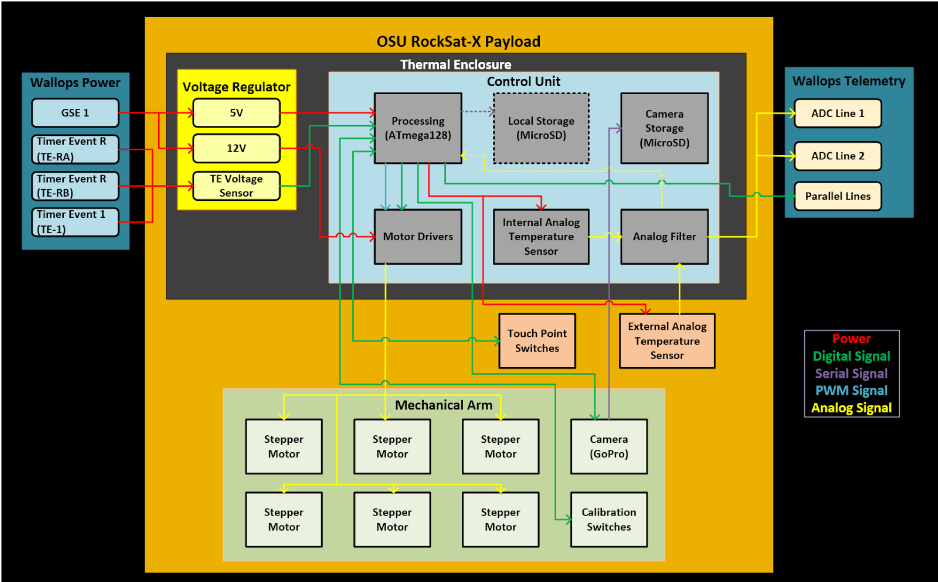
\includegraphics[width=\textwidth]{./images/ProjectDocs/functionalBlockDiagram}

\subsubsection{Flow Diagram}
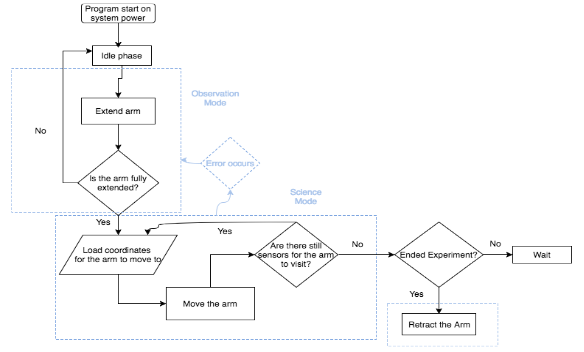
\includegraphics[width=\textwidth]{./images/ProjectDocs/flowDiagram}

\subsubsubsection{Pathing and Automation Subsystem Flow Diagram}
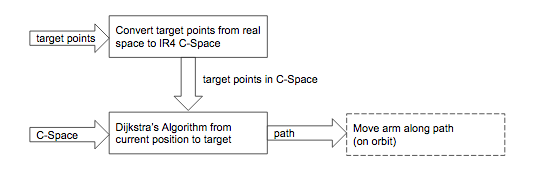
\includegraphics[width=\textwidth]{./images/ProjectDocs/pathingAndAutomationFlow}

\subsection{Hardware Requirements}
Minimum hardware requirements to run the software for the Hephaestus payload include:
\begin{itemize}
	\item{ATmega128 microcontroller}
	\item{USB ASP programmer}
\end{itemize}

\subsection{Installation Instructions}
To install the software on an ATmega128 chip, first ensure it is connected to
the computer with a USB ASP programmer. Then, from the 
\texttt{code/Hephaestus/Hephaestus} directory, run \texttt{make all}
followed by \texttt{make program}.

\subsection{Running Instructions}
The code will immediately begin running once the chip is powered on, and will
continue to run until power is lost.

\subsection{User Guides and Documentation}
\subsubsection{Program Overview}
Hephaestus is a rocketry payload made by Oregon State University for the RockSat-X program. The faculty advisor for this project is Nancy Squires. The involvement of twelve of the project contributors is part of the Senior Design classes. The Senior Design groups include two Mechanical Engineering groups, an Electrical Engineering group, and the Computer Science group. This repository is for project deliverables for the CS Senior Design class as well as any design documents, code, testing, data, and documentation generated by the Computer Science team throughout the 2016/2017 Senior Design year.

Participation and flight in the RockSat-X program is subject to revue and approval from the Colorado Space Grant Consortium. Pending this approval, the Hephaestus payload will fly in August of 2017.

\subsubsection{Mission Overview}
The Oregon State University RockSat-X team will demonstrate that an autonomous robotic arm can locate predetermined targets around the payload under microgravity conditions by using precise movements. The technical actions performed by this demonstration will illustrate a proof of concept for creating assemblies, autonomous repairs, and performing experiments in space.

\subsubsection{Repository Contents}
This section will describe the contents and structure of this repository.

\subsubsubsection{Deliverables}
The deliverables directory shall contain all deliverables for the CS Senior Design course. These deliverables are broken up into the term and assignment subdirectories. Assignments will be added through June 2017, at which point the course will conclude.

\subsubsubsection{Design Documents}
The Design Documents directory contains all design documents that we create. These shall be further organized by term and subject, pending need for organization. For the moment this shall be a place for any in progress, partial, or draft items.

\subsubsubsection{Photos}
The Photos directory shall include all photo documentation for the project, including any graphics for promotional use (such as logos or flyers).

\subsubsubsection{Presentations}
The Presentations directory shall include all presentations given by the CS team. This will include all presentations for RockSat-X program design reviews, presentations for promotional purposes, or for fundraising purposes.

\subsubsubsection{Code}
\begin{itemize}
	\item \textbf{CSpace}

	Contains the code for mapping and parsing the configuration space.

	\item \textbf{Drivers}

	Contains the drivers given to us by the Electronics team.

	\item \textbf{Hephaestus}

	Contains all the code written by the Software team to operate the \gls{payload}.

	\item \textbf{SDRead}

	Contains the code to parse telemetry files and display data in a \gls{gui}.
\end{itemize}

\subsubsection{Instructions to build}

\subsubsubsection{Before you build}
Before you can build the code for this project, make sure you have the avr-gcc 
compiler as well as an ATmega128 microchip and programmer. You can obtain a 
copy of the avr-gcc compiler from the 
\href{http://winavr.sourceforge.net/}{WinAVR suite} for Windows, or by 
installing the `avr-libc`, `binutils-avr`, `gcc-avr`, and `avrdude` packages 
from your Linux OS's package repository. In the case of OS X/macOS, ensure that 
you have version 5.11.1 of avrdude installed as the most recent version does 
not work with our implementation. The ATmega128 chip can be purchased from 
\href{https://www.microchip.com/wwwproducts/en/ATMEGA128}{Microchip's website}.
Also, be sure to have a programming board for your ATmega128 chip, which can be 
obtained from the \gls{osu} TekBot store.

\subsubsubsection{Building}
\begin{enumerate}
	\item{Navigate to the \texttt{code/Hephaestus/Hephaestus} directory.}
	\item{Run \texttt{make all} to compile the code.}
	\item{Run \texttt{make program} to program the microcontroller.}
\end{enumerate}

\section{Learning New Technology}
\subsection{Helpful Resources}
\subsubsection{Web Sites}
\begin{enumerate}
\item{\href{http://www.atmel.com/webdoc/avrlibcreferencemanual/}{Atmel AVR Libc Reference Manual}}
\item{\href{https://www.sharelatex.com/learn/}{ShareLatex Documentation}}
\item{\href{http://phobos.colorado.edu/national-programs/rs-x-2017-home}{RockSat-X Program Homepage}}
\end{enumerate}

\subsubsection{Books and Print Materials}
No books or print materials were used for this project.

\subsubsection{Faculty and Personnel}
\begin{enumerate}
\item{Dr. Nancy Squires}
\item{Dr. Bill Smart}
\end{enumerate}


\section{What We Learned}
\subsection{Helena Bales}
\subsubsection{Technical Information}
TODO

\subsubsection{Non-Technical Information}
TODO

\subsubsection{Project Work Information}
TODO

\subsubsection{Project Management Information}
TODO

\subsubsection{Team Work Information}
TODO

\subsubsection{If you could do it all over what would you do differently?}
TODO


\subsection{Amber Horvath}
\subsubsection{Technical Information}
TODO

\subsubsection{Non-Technical Information}
TODO

\subsubsection{Project Work Information}
TODO

\subsubsection{Project Management Information}
TODO

\subsubsection{Team Work Information}
TODO

\subsubsection{If you could do it all over what would you do differently?}
TODO


\subsection{Michael Humphrey}
\subsubsection{Technical Information}
TODO

\subsubsection{Non-Technical Information}
TODO

\subsubsection{Project Work Information}
TODO

\subsubsection{Project Management Information}
TODO

\subsubsection{Team Work Information}
TODO

\subsubsection{If you could do it all over what would you do differently?}
TODO



\section{Appendix 1: Essential Code}
\subsection{Pre-Processing}
\subsubsection{CSpace\_Mapping.ino}
\begin{lstlisting}[language=C]
#include <stdio.h>

//=========DEFINITIONS==================
int encA_pin1 = 6;
int encB_pin1 = 7;
long encA_ticks1 = 0;
//for polling implementation
int n = LOW;
int encA_pin1_prev = LOW;

unsigned long time;
char buffer [50];
int i = 0;

int encA_pin2 = 2;
int encB_pin2 = 4;
volatile long encA_ticks2 = 0;

int encA_pin3 = 3;
int encB_pin3 = 5;
volatile long encA_ticks3 = 0;

const float pi = 3.14;

volatile int state = HIGH;

volatile float encA_degree1 = 0;
volatile float encA_degree2 = 0;
volatile float encA_degree3 = 0;

/*
2 - Motor 1: A
3 - Motor 1: B
4 - Motor 2: A
5 - Motor 2: B
6 - Motor 3: A
7 - Motor 3: B


*/
//=========SET-UP==================
void setup() {
  // put your setup code here, to run once:
pinMode(encA_pin1, INPUT);
pinMode(encA_pin2, INPUT);
pinMode(encA_pin3, INPUT);

digitalWrite(encA_pin1, HIGH);
digitalWrite(encA_pin2, HIGH);
digitalWrite(encA_pin3, HIGH);

pinMode(13, OUTPUT);

// INIT interrups

//switch motor 1 to polling
//attachInterrupt(digitalPinToInterrupt(encA_pin1),encoderA1,RISING);
attachInterrupt(digitalPinToInterrupt(encA_pin2),encoderA2,RISING);
attachInterrupt(digitalPinToInterrupt(encA_pin3),encoderA3,RISING);

Serial.begin(9600);
}


//========= LOOP ==================
void loop() {
  // put your main code here, to run repeatedly:

  time = millis();

  //Poll innermost motor to circumvent limited number
  //of Arduino UNO interupts
  n = digitalRead(encA_pin1);
   if ((encA_pin1_prev == LOW) && (n == HIGH)) {
     if (digitalRead(encB_pin1) == LOW) {
       encA_ticks1 -= 1.0;
     } else {
       encA_ticks1 += 1.0;
     }
   } 
   encA_pin1_prev = n;

  digitalWrite(13,state);

  //if enough time has passed, print a status update
  //print status update every .5 seconds

  //output the valid configurations to Serial which will then be stored in a file
  encA_degree1 = encA_ticks1*2.25;
  encA_degree2 = encA_ticks2*2.25;
  encA_degree3 = encA_ticks3*2.25;

  Serial.println("0");
  Serial.println(encA_degree1);
  Serial.println(encA_degree2);
  Serial.println(encA_degree3);
  Serial.println(";");

  delay(500);
}

//Arduino UNO only has two interupts
//Switch innermost motor to polling

//void encoderA1(){
//  state=!state;
//  if(digitalRead(encB_pin1)==HIGH){
//    encA_ticks1=encA_ticks1+1.0;
//  }else{
//    encA_ticks1=encA_ticks1-1.0;
//  }
//  }

void encoderA2(){
  state=!state;
  if(digitalRead(encB_pin2)==HIGH){
    encA_ticks2=encA_ticks2+1.0;
  }else{
    encA_ticks2=encA_ticks2-1.0;
  }
}
  
void encoderA3(){
  state=!state;
  if(digitalRead(encB_pin3)==HIGH){
    encA_ticks3=encA_ticks3+1.0;
  }else{
    encA_ticks3=encA_ticks3-1.0;
  }
  }

\end{lstlisting}
\subsubsection{parser.cpp}
\begin{lstlisting}[language=C++]
#include <stdio.h>
#include <stdlib.h>
#include <iostream>
#include <fstream>
#include <string>
#include <cstring>
#include <time.h>
#include <unistd.h>
#include <math.h>

using namespace std;

/************************************************************************************************
 * Program: C-Space Data Parser
 * Author: Helena Bales
 * Date: April 12th, 2017
 * Description: A C++ implementation of a parser for the Hephaestus Configuration Space data. The 
 * 	parser creates a 4-D array of boolean values with a 0 representing a valid configuration 
 * 	and a 1 representing an invalid configuration.
 * Input: ./test1/data1 - Hephaestus C-Space data as defined in project docs
 * Output: ./cspace.out - Output file containing boolean data from 37x37x37x37 array
 ***********************************************************************************************/

int main() {
	char* myFile;
	ifstream sourceFile;
	ofstream outfile;
	string line;

	int accuracyFactor = 10;
	int MAX_ANGLE = 360;
	int x = MAX_ANGLE/accuracyFactor;
	int a, b, c, d;
	float af, bf, cf, df;
	bool endOfFile = 0;

	unsigned char CSpace[37][37][37][37];

	//init C-Space with 1's
	for(a=0; a<x; a++) {
		for(b=0; b<x; b++) {
			for(c=0; c<x; c++) {
				for(d=0; d<x; d++) {
					CSpace[a][b][c][d] = 255;
				}
			}
		}
	}

	//open file
	myFile = "./test1/data1";
	sourceFile.open(myFile);
	
	//loop for length of file
	while(!endOfFile) {
		//read 5 lines from the file
		
		//line 1 == a
		getline(sourceFile, line);
		af = stof(line, NULL);
		//cout << "af = " << af << endl; //FOR TESTING

		//line 2 == b
		getline(sourceFile, line);
		bf = stof(line, NULL);
		//cout << "bf = " << bf << endl; //FOR TESTING

		//line 3 == c
		getline(sourceFile, line);
		cf = stof(line, NULL);
		//cout << "cf = " << cf << endl; //FOR TESTING

		//line 4 == d
		getline(sourceFile, line);
		df = stof(line, NULL);
		//cout << "df = " << df << endl; //FOR TESTING

		//line 5 == ; divider between coordinates
		getline(sourceFile, line);
		//cout << ";" << endl;

		//convert negative degrees to corresponding positive angle
		if(af < 0) {
			af = 360 + af;
		}

		if(bf < 0) {
			bf = 360 + bf;
		}

		if(cf < 0) {
			cf = 360 + cf;
		}

		if(df < 0) {
			df = 360 + df;
		}

		//convert to ints
		a = floor(af/10);
		b = floor(bf/10);
		c = floor(cf/10);
		d = floor(df/10);

		//check floored values against original FOR TESTING
		cout << a << "/" << af << " - " << b << "/" << bf << " - " << c << "/" << cf << " - " << d << "/" << df << endl;

		//mark array[a][b][c][d] = 0
		CSpace[a][b][c][d] = 0;

		//check if eof has been reached
		if(sourceFile.eof()) {
			cout << "Reached eof - check 3" << endl;
			endOfFile = 1;
		}

		//check if eof has been reached
		if(sourceFile.peek() == 10) {
			cout << "Reached eof - check 2" << endl;
			endOfFile = 1;
		}
	}

	//close source file
	if(sourceFile.is_open()) {
		sourceFile.close();
	}

	/*
	//print array
	for(a=0; a<1; a++) {
		for(b=0; b<37; b++) {
			for(c=0; c<37; c++) {
				for(d=0; d<37; d++) {
					cout << CSpace[a][b][c][d];
				}
				cout << endl;
			}
			cout << endl;
			cout << endl;
		}
	}
	*/

	//store array in file
	outfile.open("cspace");
	for(a=0; a<x; a++) {
		for(b=0; b<x; b++) {
			for(c=0; c<x; c++) {
				for(d=0; d<x; d++) {
					outfile << (int)CSpace[a][b][c][d];
				}
			}
		}
	}

	/*
	//store 0 locations in file for plotting
	outfile.open("cspacePlotData");
	for(a=0; a<x; a++) {
		for(b=0; b<x; b++) {
			for(c=0; c<x; c++) {
				for(d=0; d<x; d++) {
					if(CSpace[a][b][c][d] == 0){
						outfile << b << " " << c << " " << d 
							<< endl;

					}
				}
			}
		}
		outfile << "\n";
	}
	*/
	
}

\end{lstlisting}
\subsubsection{convert.cpp}
\begin{lstlisting}[language=C++]
#include <stdio.h>
#include <stdlib.h>
#include <iostream>
#include <fstream>
#include <string.h>
#include <cstring>
#include <time.h>
#include <unistd.h>
#include <math.h>

using namespace std;

/************************************************************************************************
 * Program: Target point converter
 * Author: Helena Bales (Inverse Kinematics by Brett Moffatt)
 * Date: May 17th, 2017
 * Description: For the RockSat-X Hephaestus payload. Converts our target points from cartesian 
 * 	form into a representation within the configuration space. This is accomplished through 
 * 	Inverse Kinematics with theta0 isolated to four discrete values, allowing us to resolve 
 * 	the results of IK from a 4D area in the configuration space to four possible solutions,
 * 	of which at least one must be marked as 0 in the cspace.
 * Input: ./targets - A text document containing one target (in the form: x y z) per line, in 
 * 		cartesian form
 * Output: ./thetaTargets - A text document containing one target per line (in the form: 
 * 	theta0 theta1 theta2 theta3), where theta0-3 refers to the rotational angle from the 
 * 	defined normal
 ***********************************************************************************************/

/************************************
 * theta1 = roll = {0, 90, 180, 270}
 * theta2 = yaw = tan-1(yo/xo)
 * theta3 = pitch1
 * theta4 = pitch2
 ***********************************/

int main() {
	char* myFile;
	ifstream sourceFile;
	ofstream outfile;
	char line[24];
	char* tokens;

	int xo, yo, zo;	//real target point
	int theta0, theta1, theta2, theta3; //cspace target point
	double l1, l2; //arm segment lengths
	double k1, k2, gamma; //variables for calculating pitch
	double t, b, fraction1, pt1, pt2; //some more variables for calculations
	bool endOfFile = 0; //marker for eof

	//define arm lengths
	l1 = 3.99;
	l2 = 4.49;

	//open the file of targets
	myFile = "./targets";
	sourceFile.open(myFile);

	//open the file for theta targets
	myFile = "./thetaTargets";
	outfile.open(myFile);


	while(!endOfFile) {
		//read a line
		sourceFile.getline(line, 24);

		//break the line on spaces
		tokens = strtok(line, " ");

		//store the values as integers
		xo = stoi(tokens);
		tokens = strtok(NULL, " ");

		yo = stoi(tokens);
		tokens = strtok(NULL, " ");

		zo = stoi(tokens);
		tokens = strtok(NULL, " ");

		//check if it is eof
		if(sourceFile.eof() || sourceFile.peek() == 10) {
			endOfFile = 1;
			cout << "end of file reached" << endl;
		}

		//calculate variables
		t = (xo*xo) + (yo*yo) - (l1*l1) - (l2*l2);
		b = 2 * l1 * l2;
		fraction1 = t/b;
		pt1 = sqrt(1 - (fraction1 * fraction1));
		pt2 = fraction1;

		//calcualte theta2
		theta2 = atan2(zo, sqrt((yo*yo) + (xo*xo)));

		//calculate k1, k2, and gamma
		k1 = l1 + (l2 * cos(theta2));
		k2 = l2 * sin(theta2);
		gamma = atan2(k1, k2);

		//calculate theta0, theta1, theta3
		theta1 = atan(yo/xo);
		theta3 = atan2(yo, xo) - gamma;
		theta0 = 0; //TODO move this motor to change the plane

		//print the thetas to the file
		outfile << theta0 << " " << theta1 << " " << theta2 << " " << theta3 << " " << endl;

	}

	//close the file
	if(sourceFile.is_open()) {
		sourceFile.close();
	}

	//close the file
	if(outfile.is_open()) {
		outfile.close();
	}


	return 0;
}
\end{lstlisting}

\subsubsection{pathing.cpp}
TODO
\begin{lstlisting}[language=C++]
\end{lstlisting}

\subsection{Data Storage}
\subsubsection{SDRead.py}
\begin{lstlisting}[language=Python]
import matplotlib.pyplot as plt
import sys

if len(sys.argv) != 2:			# Make sure filename is specified on command line
	print("No file specified.")	
	print("USAGE:", sys.argv[0], "<filename>")
	sys.exit(1)

temps = []							# Create an empty list of temperatures

with open(sys.argv[1], "br") as f:	# Open output file for binary reading
	data = bytes(f.read(3))			# Read three bytes
	while data != bytes(b""):		# Make sure we have input (i.e. not EOF)
		num = (data[0] * pow(2, 8))	# Load the most significant byte
		num += (data[1])			# Load the least significant byte
		temps.append(num)			# Store the number in the array
		data = bytes(f.read(3))		# Get thee next three bytes
	
scaled = [(i/(2**10)) for i in temps] # Scale the temperature values to between 0-1
plt.plot(scaled)					# Create the plot
plt.ylabel("Relative temperature")	# Always label your axises
plt.xlabel("Sample number")			
plt.show()							# Display the plot
\end{lstlisting}

\subsubsection{telemetry.c}
\begin{lstlisting}[language=C]
/*
 * telemetry.c
 *
 * Created: 1/18/2017 10:44:49 AM
 *  Author: Michael Humphrey
 */ 

#include "telemetry.h"
#include "RSXAVRD.h"
#include <avr/eeprom.h>
#include <string.h>

uint16_t current_address;

void telemetry_init(void) {
	current_address = eeprom_read_word(0);
	if (current_address == 0xFFFF) {
		current_address = 2;
	}
}

// Sends a code with the predefined TELEMETRY_TIME constant.
void inline telemetry_send_code(uint8_t code) {
	send_code(code, TELEMTRY_TIME);
}

// Log a message to the EEPROM
void eeprom_log(char* message) {
	eeprom_update_block(message, (void *) (uint16_t) current_address, strlen(message)+1);
	current_address += strlen(message)+1;
	eeprom_update_word(0, current_address);
}


// Log a message to the SD card - DEPRECATED
/*
void SD_log(char* message) {
	// Write elapsed time to SD card
	char *result = (char*) malloc(6*sizeof(char)); // Max value of get_time() is 65535, which is 5 characters, plus 1 for null terminator

	if (result == NULL)
		return;

	itoa(get_time(), result, 10);
	// Write result string to SD card
	free(result);

	// Write separator to SD card

	// Write message to SD card

	// Write line terminator to SD card
}
*/
\end{lstlisting}

\subsection{Main}
\subsubsection{main.c}
\begin{lstlisting}[language=C]
/*
 * Hephaestus.c
 *
 * Created: 1/17/2017 6:05:07 PM
 * Author : Michael Humphrey
 */ 

#include <avr/io.h>
#include "phases.h"
#include "RSXAVRD.h"
#include "retract.h"


int main(void)
{
	// Pin configuration
	AVR_init();

	uint8_t status = 0;

	//timer_counter_enable(1,1); // code that enables timer event - Jon says Michael wanted this?

	timer_event_enable(0,1); // enables timer event line 0

	timer_event_enable(1,1); // enables timer event line 1

    /* Replace with your application code */
    while (1) 
    {
		// Phase 1: Idle
		status = idle();

		// Phase 2: Observation
		status = observation();

		// Phase 3: Science
		status = science();
		if (status != 0) { // if our arm is not calibrated i.e. collapsed and in home position...
			retract(); // turn off all motors and retract into a safe position
		}

		// Phase 4: Off
		status = off();
		// Under normal circumstances, off never returns.
		// Off only returns if there was an error.

		// Phase 5: Safety
		status = safety();
    }
}
\end{lstlisting}

\subsubsection{phases.h}
\begin{lstlisting}[language=C]
/*
 * phases.h
 *
 * Created: 1/20/2017 3:36:58 PM
 *  Author: Michael Humphrey
 */ 


#ifndef PHASES_H_
#define PHASES_H_

int idle(void);			// Phase 1
int observation(void);	// Phase 2
int science(void);		// Phase 3
int off(void);			// Phase 4
int safety(void);		// Phase 5
void retract(void);  // retract phase

#endif /* PHASES_H_ */
\end{lstlisting}

\subsubsection{Modes of Operation}
\subsubsubsection{idle.c}
\begin{lstlisting}[language=C]
/*
 * idle.c
 *
 * Created: 1/20/2017 3:36:32 PM
 *  Author: Michael Humphrey
 */

#include "RSXAVRD.h"
#include <avr/io.h>
#include <avr/interrupt.h>
#include "telemetry.h"

uint8_t ready = 0;

ISR(INT6_vect) {
	ready = 1;
}

 // First phase of payload deployment. Wait for TE-R lines to go high, then return.
 int idle(void) {
	
	// Infinite loop until receive signal to start


	while (!ready) {}

	eeprom_log("idle phase complete");

	return 0;
}
\end{lstlisting}

\subsubsubsection{observation.c}
\begin{lstlisting}[language=C]

/*  observation.c
 *  Created: 1/22/2017 5:12:25 PM
 *  Author: Amber Horvath
 */

#include <avr/io.h>
#include "phases.h"
#include "RSXAVRD.h"
#include "telemetry.h"
#include "MOTOR_DEF.h"

int observation(){

     
      camera_enable(POWER_ON); // turns on camera

      motor_pwr(MOTOR_CAMERA, POWER_ON); // power on the motor for the camera

      motor_dir(MOTOR_CAMERA, CLOCKWISE); // set the camera to move clockwise

      motor_step(MOTOR_CAMERA, DEGREES_TO_STEPS(180), 1, 85);

      _delay_ms(500);

      motor_dir(MOTOR_CAMERA, COUNTER_CLOCKWISE);

      motor_step(MOTOR_CAMERA, DEGREES_TO_STEPS(360), 1, 85);

      _delay_ms(500);

      motor_dir(MOTOR_CAMERA, CLOCKWISE);

      motor_step(MOTOR_CAMERA, DEGREES_TO_STEPS(180), 1, 85);

      _delay_ms(500); 

      telemetry_send_code(OBSERVATION_PHASE); // let us know we finished Observation mode

      eeprom_log("observation phase complete");

      return 0;


}

\end{lstlisting}

\subsubsubsection{science.c}
\begin{lstlisting}[language=C]
#include <avr/io.h>
#include "phases.h"
#include "RSXAVRD.h"
#include "telemetry.h"
#include <avr/interrupt.h>
#include <util/delay.h>
/*
* Design of science phase: arm will move to touch sensor and press it. Upon moving the arm to the location, we will
* check whether the touch sensor was pressed and change our status to represent whether or not it was pressed.
* We will also write a code over the telemetry lines to represent whether or not the touch sensor was pressed.
*/

int science(){
	int status = 0;
	int M1_POS, M2_POS, M3_POS, M4_POS;
	int M1_NXT, M2_NXT, M3_NXT, M4_NXT;
	int M1_DIF, M2_DIF, M3_DIF, M4_DIF;
	int M1_STP, M2_STP, M3_STP, M4_STP;
	int scale_factor = 0.225;
	char path_step;

	//TODO reference CSpace in program memory (the address of a 4D array in program memory)
	char**** cspace;
		
	// init motor values to 0
	M1_POS = 0;
	M2_POS = 0;
	M3_POS = 0;
	M4_POS = 0;

	// turn on camera
	camera_enable(1);

	// power on motors
	motor_pwr(1, 1);
	motor_pwr(2, 1);
	motor_pwr(3, 1);
	motor_pwr(4, 1);

	//repeat for length of path
	while(1) {
		//set motor direction to be forward
		motor_dir(1, 0);
		motor_dir(2, 0);
		motor_dir(3, 0);
		motor_dir(4, 0);
		
		//find the next point in the path
		path_step = cspace[M1_POS][M2_POS][M3_POS][M4_POS];

		//set the lower and upper bounds for the loops so only indeces 
		//in range are checked
		if(M1_POS == 0) { sw = 0; } else { sw = -1; }
		if(M2_POS == 0) { sx = 0; } else { sx = -1; }
		if(M3_POS == 0) { sy = 0; } else { sy = -1; }
		if(M4_POS == 0) { sz = 0; } else { sz = -1; }

		if(M1_POS == 36) { ew = 1; } else { ew = 2; }
		if(M2_POS == 36) { ex = 1; } else { ex = 2; }
		if(M3_POS == 36) { ey = 1; } else { ey = 2; }
		if(M4_POS == 36) { ez = 1; } else { ez = 2; }


		//check each of the neighboring points
		for(int w=sw; w<ew; w++) {
			for(int x=sx; x<ex; x++) {
				for(int y=sy; y<ey; y++) {
					for(int z=sz; z<ez; z++) {
						if(cspace[M1_POS+w][M2_POS+x][M3_POS+y][M4_POS+z] == path_step + 1) {
							M1_NXT = M1_POS + w;
							M2_NXT = M2_POS + x;
							M3_NXT = M3_POS + y;
							M4_NXT = M4_POS + z;
							break;
						}
					}
				}
			}
		}

		if(M1_NXT == M1_POS && M2_NXT == M2_POS && M3_NXT == M3_POS && M4_NXT == M4_POS) {
			//end of path has been reached
			//TODO send eop telemetry signal
			return 0;
		}

		//change _NXT values to be less than 360
		if(M1_NXT > 359) {
			M1_NXT = M1_NXT - 359;
		}

		if(M2_NXT > 359) {
			M2_NXT = M2_NXT - 359;
		}

		if(M3_NXT > 359) {
			M3_NXT = M3_NXT - 359;
		}

		if(M4_NXT > 359) {
			M4_NXT = M4_NXT - 359;
		}
		
		// calculate change in each motor (in degrees)
		M1_DIF = M1_NXT - M1_POS;
		M2_DIF = M2_NXT - M2_POS;
		M3_DIF = M3_NXT - M3_POS;
		M4_DIF = M4_NXT - M4_POS;

		// reverse motor direction for negative difference
		if(M1_DIF < 0) {
			motor_dir(1, 1);
			M1_DIF = M1_DIF * -1;
		}

		if(M2_DIF < 0) {
			motor_dir(2, 1);
			M2_DIF = M2_DIF * -1;
		}

		if(M3_DIF < 0) {
			motor_dir(3, 1);
			M3_DIF = M3_DIF * -1;
		}

		if(M4_DIF < 0) {
			motor_dir(4, 1);
			M4_DIF = M4_DIF * -1;
		}

		// convert degress to steps
		M1_STP = M1_DIF / scale_factor;
		M2_STP = M2_DIF / scale_factor;
		M3_STP = M3_DIF / scale_factor;
		M4_STP = M4_DIF / scale_factor;

		// move each motor that many steps
		motor_step(1, M1_STP, 28, 99);
		motor_step(2, M2_STP, 28, 99);
		motor_step(3, M3_STP, 28, 99);
		motor_step(4, M4_STP, 28, 99);

		// set the current position
		M1_POS = M1_NXT;
		M2_POS = M2_NXT;
		M3_POS = M3_NXT;
		M4_POS = M4_NXT;

		if(touch_sensor_check() == 0x01){
			telemetry_send_code(TOUCH_SENSOR_1_ENGAGED); // For now, always send TOUCH_SENSOR_1_ENGAGED.
		}

		// code to return arm to callibrated "home" position
		if(get_calibration_status() != 0x01){ // or whichever motor refers to the home position
			status = 1;
		}

	}

	return status;

}
\end{lstlisting}

\subsubsubsection{retract.c}
\begin{lstlisting}[language=C]
#include <avr/io.h>
#include <avr/interrupt.h>
#include <util/delay.h>
#include "RSXAVRD.h"
#include "phases.h"
#include "retract.h"
#include "MOTOR_DEF.h"
#include "telemetry.h"

uint8_t plate_retracted_flg; // flag to keep track of plate's position

ISR(INT5_vect){
	
	if(plate_retracted_flg == 0x00){
		retract();
	}

}

void retract(){ 

	motor_pwr(MOTOR_DECK_PLATE, POWER_ON);
	
	_delay_ms(500); // delay for motor after powering on

	motor_pwr(MOTOR_CAMERA, POWER_OFF); // turn off all other motors
	motor_pwr(MOTOR_DECK_ARM, POWER_OFF);
	motor_pwr(MOTOR_PAN, POWER_OFF);
	motor_pwr(MOTOR_SHOULD, POWER_OFF);
	motor_pwr(MOTOR_ELB, POWER_OFF);

	camera_enable(POWER_OFF); 
	
	motor_dir(MOTOR_DECK_PLATE, COUNTER_CLOCKWISE); // rotates the deck plate to 

	motor_step(MOTOR_DECK_PLATE, 1650, 28, SPEED + 19); // the amount of steps needed to pull the arm back in

	eeprom_log("deck plate has been retracted");

	plate_retracted_flg = 0x01;


}

void extend(){

	motor_pwr(MOTOR_DECK_PLATE, POWER_ON); // powers on deck plate motor

	_delay_ms(500); // delays to allow motor to power on

	motor_dir(MOTOR_DECK_PLATE, CLOCKWISE); // push the deck plate out

	motor_step(MOTOR_DECK_PLATE, 1650, 28, SPEED + 19); // the amount of steps needed to move the deck plate at a good speed

	plate_retracted_flg = 0x00; // plate is NOT retracted


}
\end{lstlisting}

\subsubsubsection{safety.c}
\begin{lstlisting}[language=C]
/* safety.c
 * 
 * Created by: Amber Horvath
 * Date Created: 1/22/17 5:36:47
 *
 *
 */

#include <avr/io.h>
#include "phases.h"
#include "retract.h"
#include "telemetry.h"

int safety(void){
    
	eeprom_log("in safety - attempting retract");

    retract();

    while(1){}; // abort mission, we are hanging here

}
\end{lstlisting}

\subsubsubsection{off.c}
\begin{lstlisting}[language=C]
#include "telemetry.h"

int off(void) {

	eeprom_log("power off");

	while(1){};

	// This return statement should never be reaches, so return error.
	return 1;
}
\end{lstlisting}


\section{Appendix 2: Other Documents}
\subsection{Mission Logos}

\includegraphics[width=\textwidth]{./images/logo}
\begin{center}
Simple Mission Logo for shirts and the like.
\end{center}

\subsection{Team Photos}
\subsubsection{All Team Photo}
\includegraphics[width=\textwidth]{./images/AllTeam}
\begin{center}
From left to right,
\end{center}

\subsubsection{Software Team Photo}
\begin{center}
From left to right, Michael Humphrey, Helena Bales, Amber Horvath, and James
\end{center}

\subsection{CAD Models}
\subsubsection{Front View}
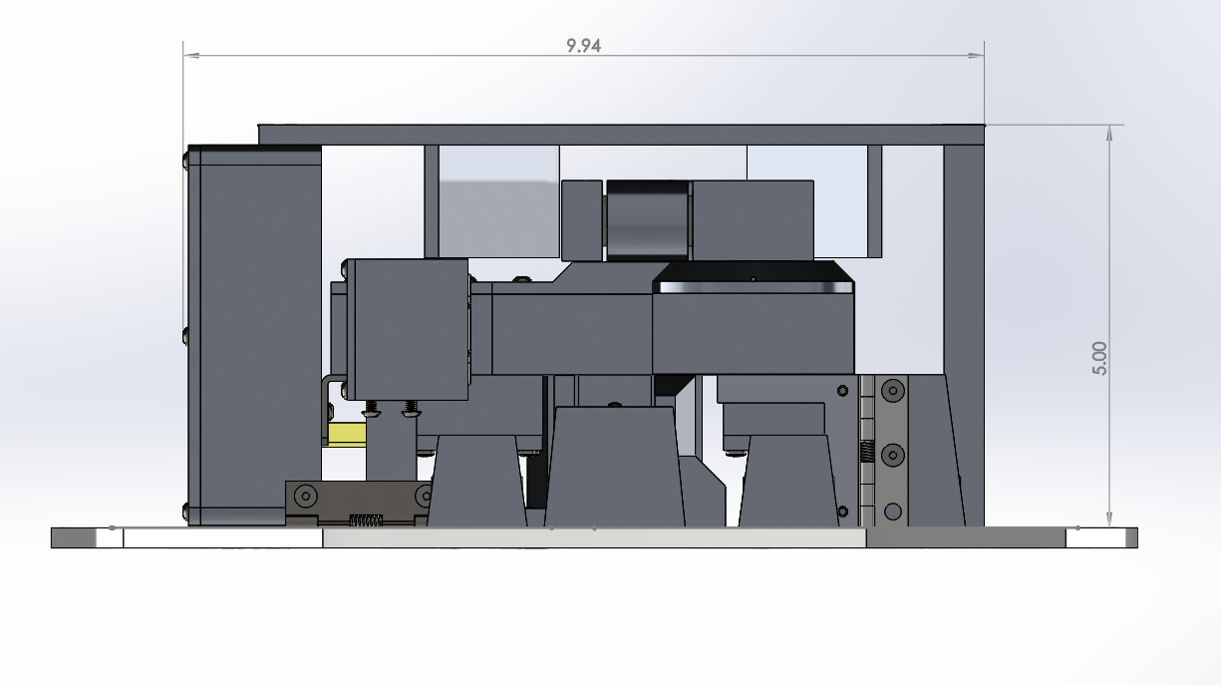
\includegraphics[width=\textwidth]{./images/CAD/FRONT}
\subsubsection{Back View}
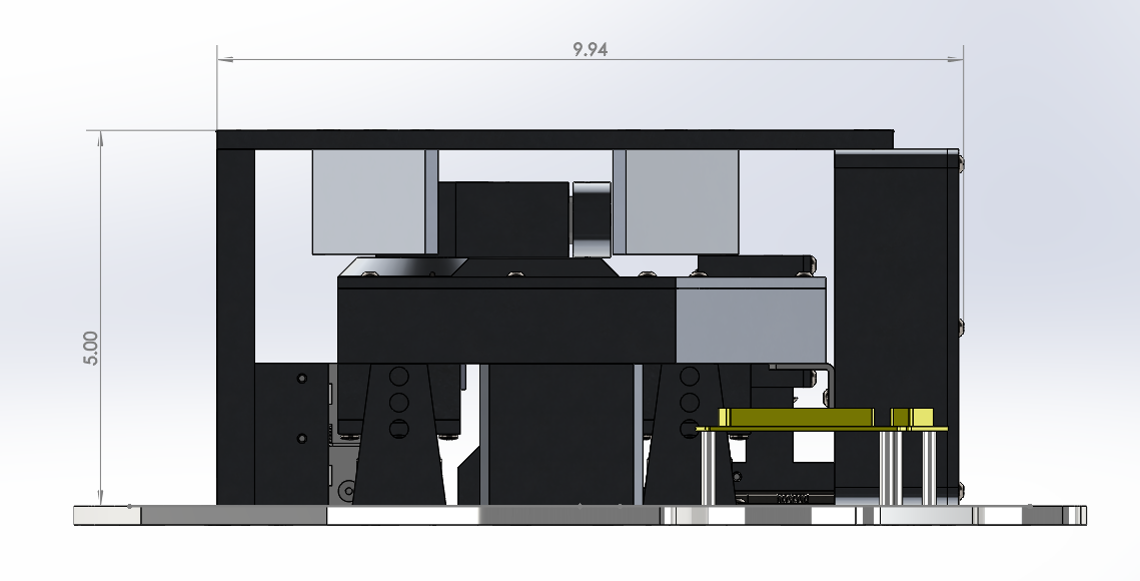
\includegraphics[width=\textwidth]{./images/CAD/BACK}
\subsubsection{Right View}
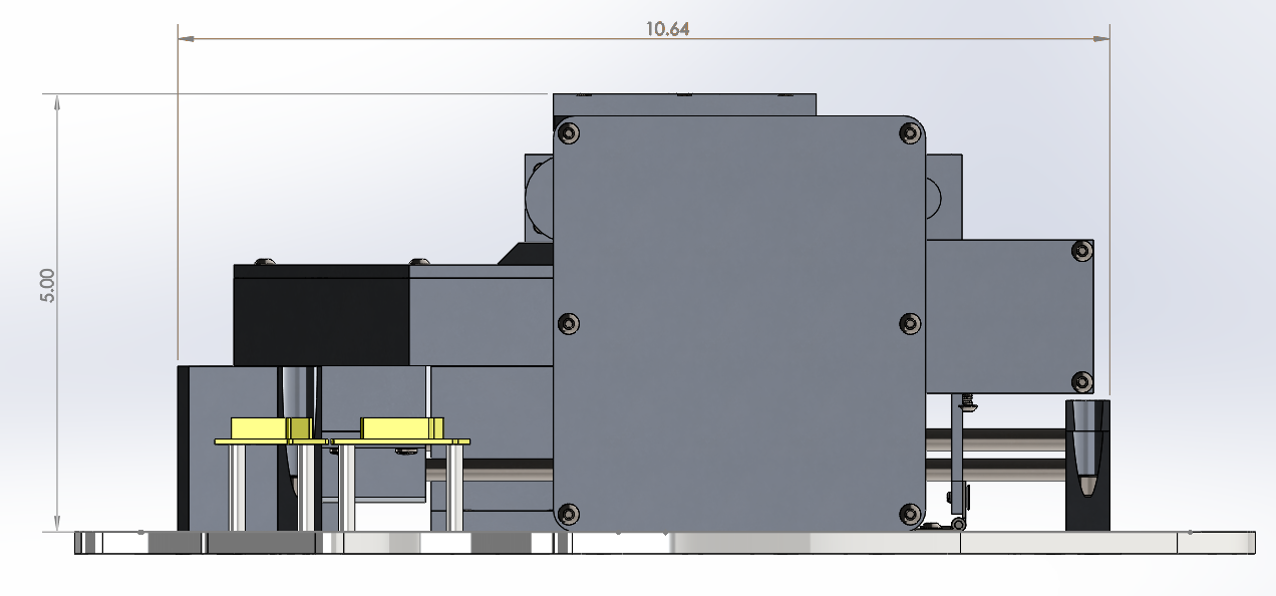
\includegraphics[width=\textwidth]{./images/CAD/RIGHT}
\subsubsection{ISO 1 View}
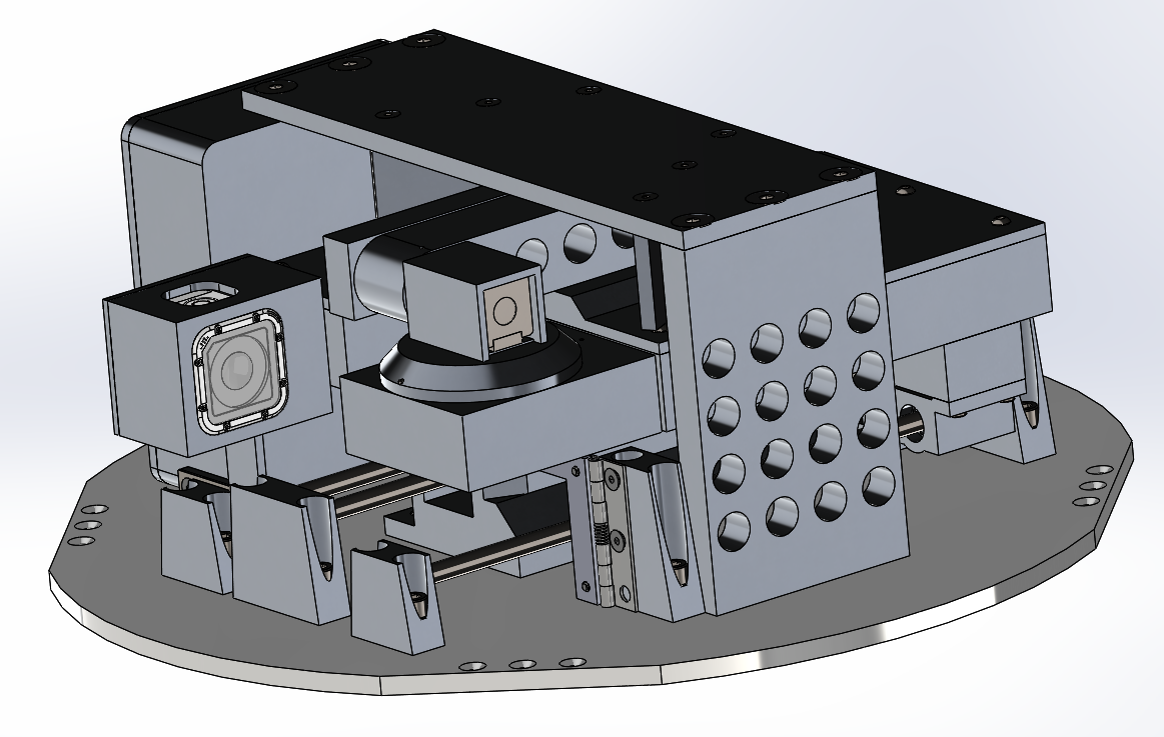
\includegraphics[width=\textwidth]{./images/CAD/ISO_1}
\subsubsection{ISO 2 View}
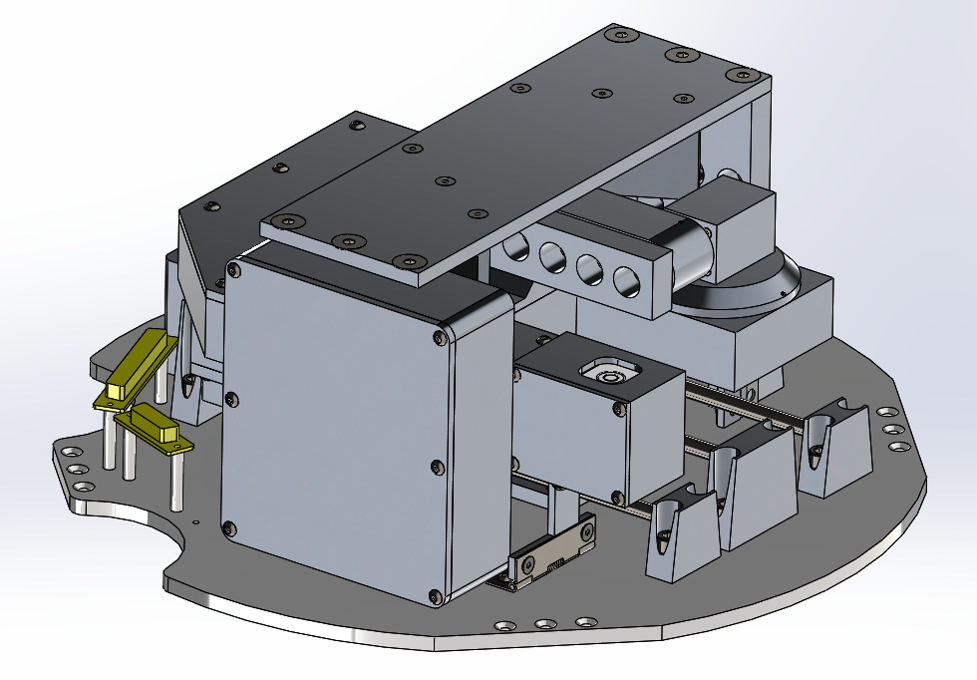
\includegraphics[width=\textwidth]{./images/CAD/ISO_2}
\subsubsection{ISO 3 View}
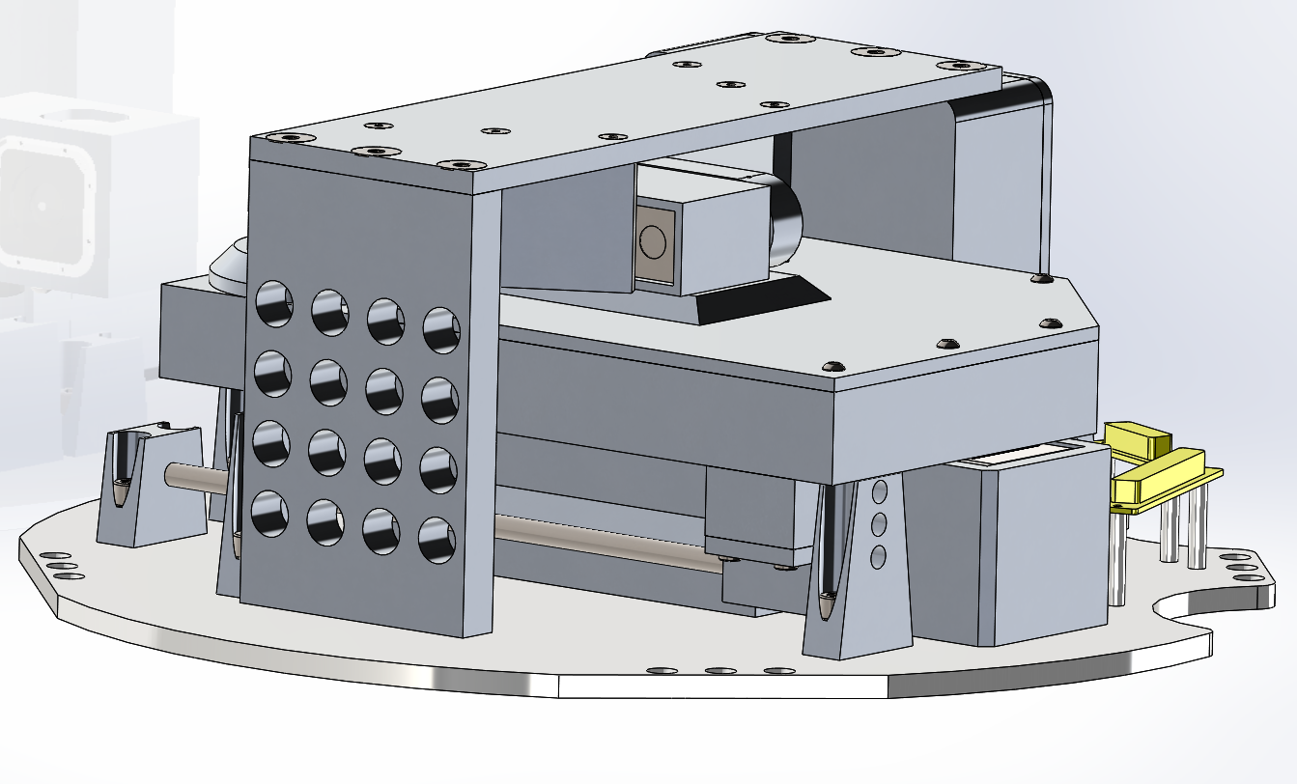
\includegraphics[width=\textwidth]{./images/CAD/ISO_3}
\subsubsection{ISO 4 View}
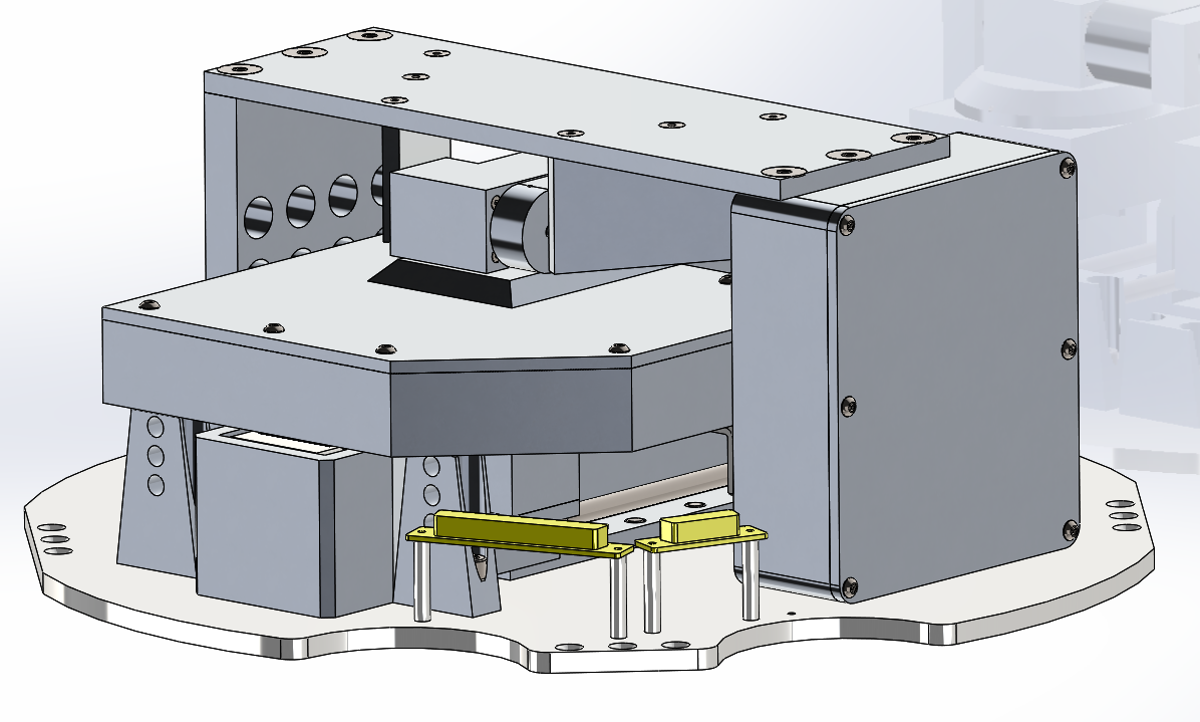
\includegraphics[width=\textwidth]{./images/CAD/ISO_4}
\subsubsection{Left View}
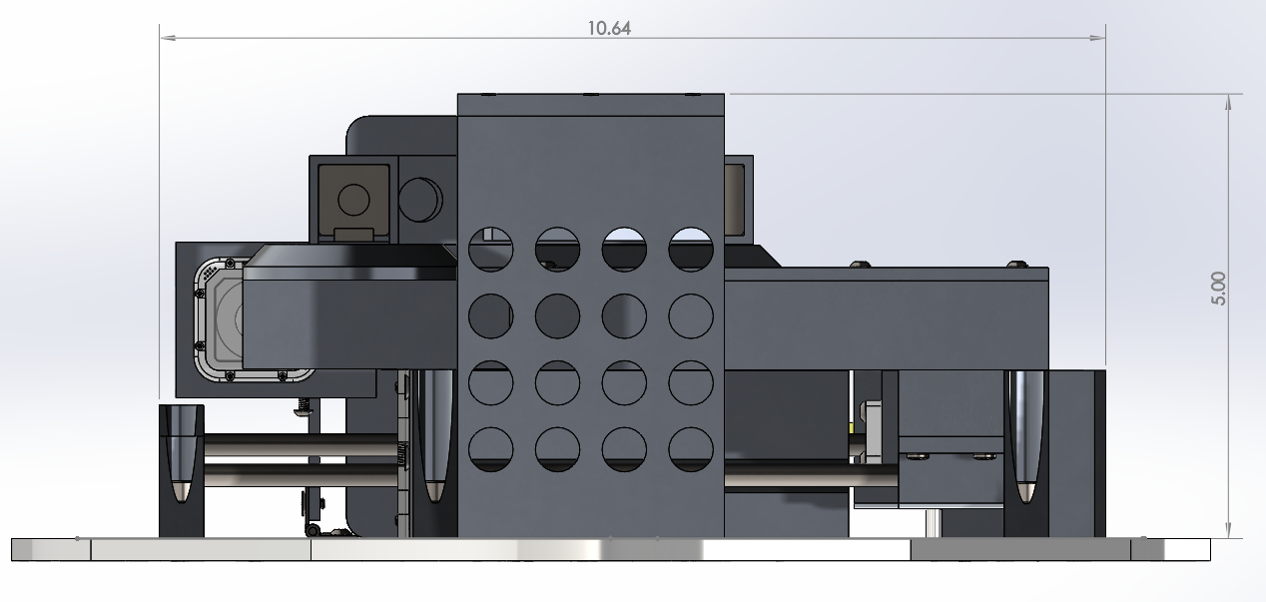
\includegraphics[width=\textwidth]{./images/CAD/LEFT}
\subsubsection{Left Fully Deployed View}
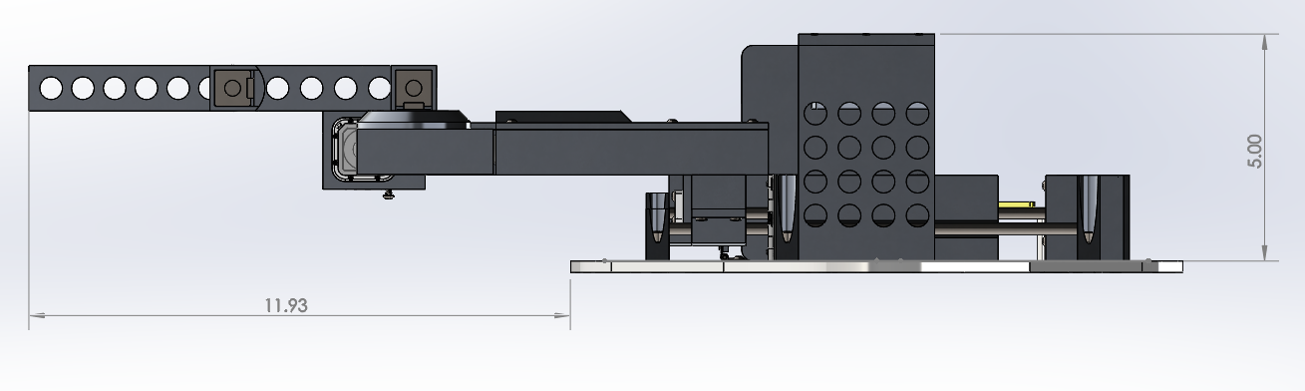
\includegraphics[width=\textwidth]{./images/CAD/LEFT_DEPLOYED_FULL}
\subsubsection{Top View}
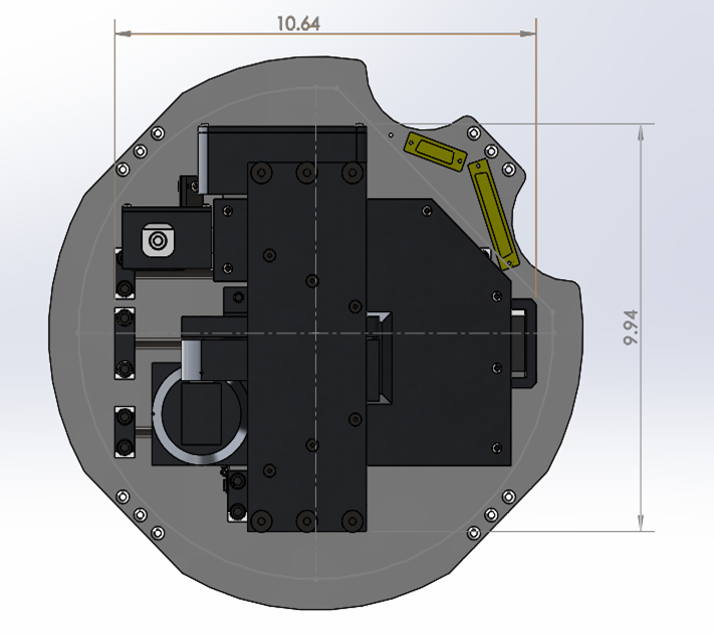
\includegraphics[width=\textwidth]{./images/CAD/TOP}
\subsubsection{Top Deployed View}
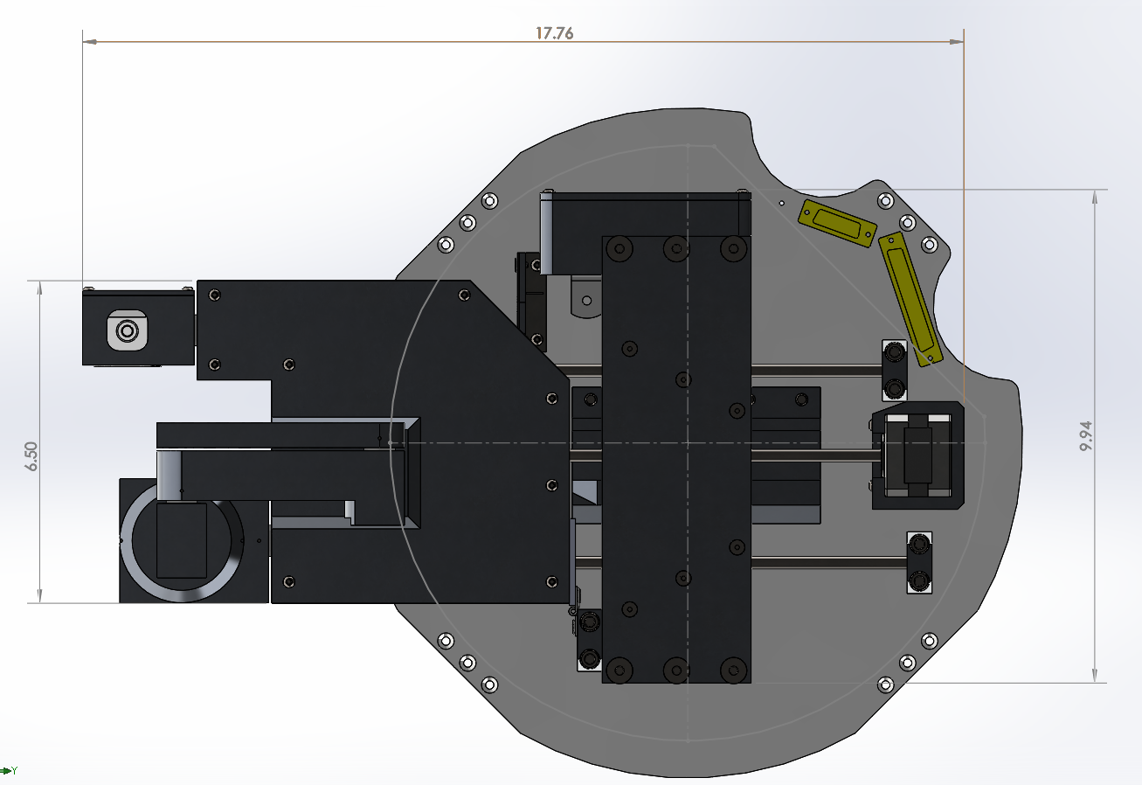
\includegraphics[width=\textwidth]{./images/CAD/TOP_DEPLOYED}
\subsubsection{Top Deployed Angle View}
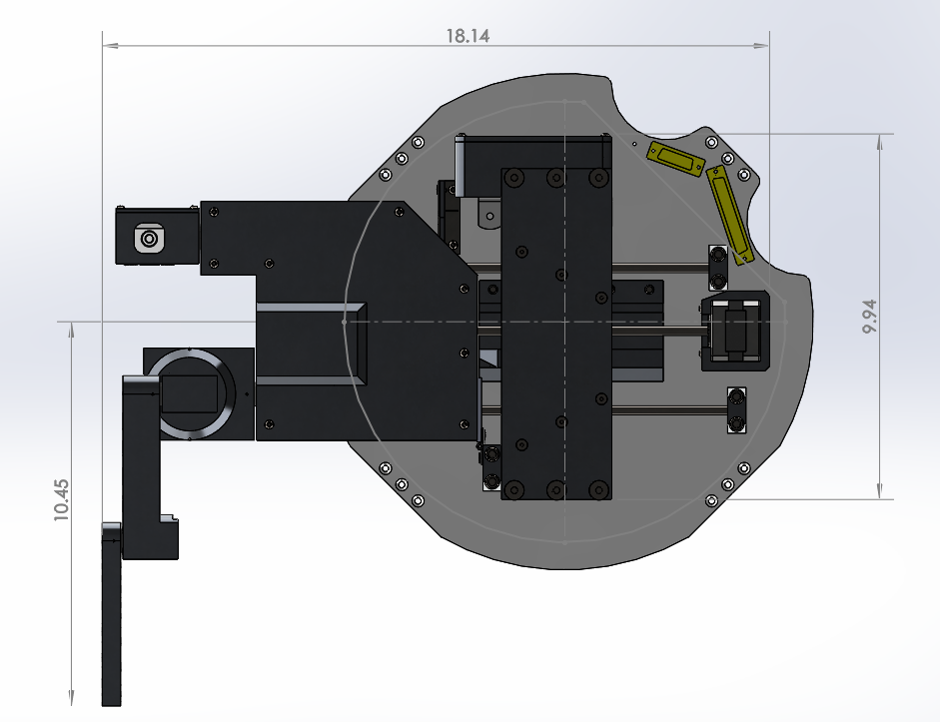
\includegraphics[width=\textwidth]{./images/CAD/TOP_DEPLOYED_ANGLE}
\subsubsection{Top Fully Deployed View}
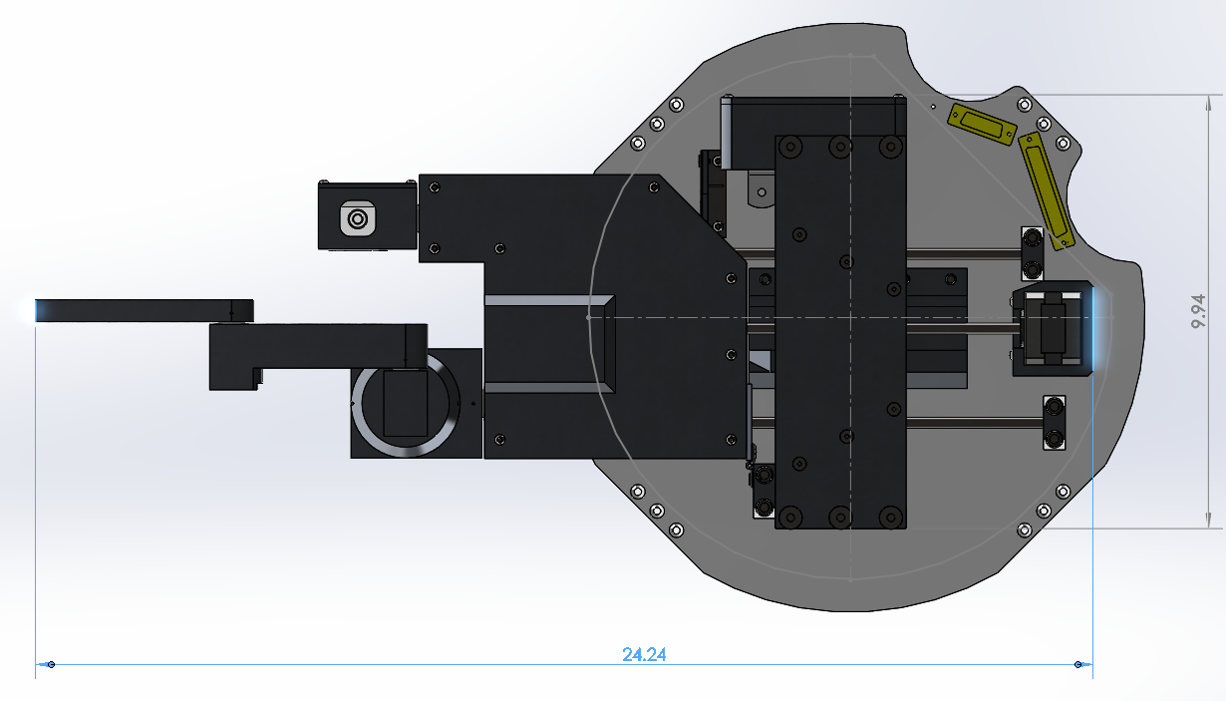
\includegraphics[width=\textwidth]{./images/CAD/TOP_DEPLOYED_FULL}

\subsection{Launch Compliance}
\subsection{Budget}


\section{Glossary}
\glsaddall
\printglossaries

\end{document}
